% !TeX spellcheck = en_US
\chapter{Feature representation of the signal domain}
\label{Chap:LLFs}
In order to develop systems that allow the users to access large music libraries, it is crucial to define and formalize the problem from the perspective of the content, i.e., the signal domain. The signal domain involves three main levels of information: the physical level, which is related to the origin and propagation of the audio wave and can be analyzed with signal processing techniques; the physiological perceptual level, which concerns how the sound is perceived by the auditory system; and the musical level that describes musicological aspects. In this Chapter we  present an overview of the state of the art needed to formalize the audio signal domain.

The MIR community developed and designed several techniques to describe the signal domain by automatically extracting features from the audio signal. Such features describe different aspects of the sound at various levels of abstraction, from those related to the energy, the spectrum or the timbre, to those regarding musical aspects of the music performance. A description of all the features employed in Music Information Retrieval is beyond the scope of this work, and in the following Sections we discuss the most popular features and those that we use throughout the thesis.

In Section \ref{sec:LLFs:hand-crafted}, we describe the so-called \textit{hand-crafted} and \textit{model-based} features, that are manually designed by scientists by means of exact mathematical formulations or of perceptual/musicological models, respectively. These features are usually divided into low-level features, that capture a specific characteristics of the audio signal by means of the exact mathematical formulations, and mid-level features that make use of the musicological aspects of the songs. For the sake of brevity, in the following discussion we will refer to both kind of features as hand-crafted features, since the perceptual or musicological models of the model-based features have been manually designed as well. 

In order to better explore the potential of such features, in Section \ref{sec:NMP} we present our research activity on Networked Music Performance, where the design of a network architecture benefits from a feature-based analysis of the (music) signal domain of the problem. In this study, we make use of both spectral low-level features captured from the audio signal and rhythmic mid-level features extracted from the scores of the corresponding musical pieces. This study was published in the Journal of Audio Engineering Society \cite{Rottondi2015}.

Finally, in Section \ref{sec:LLFs:learned}, we describe the so-called \textit{learned} features, which are automatically extracted by means of deep learning techniques, and we focus on the deep architecture we used in our works. %We also present a brief overview of deep learning techniques from the state of the art that have been used to extract a representation of the music signals.


\section{Hand-Crafted and Model-Based Features}\label{sec:LLFs:hand-crafted}
When analyzing a problem, it is important to understand which aspects are more useful to characterize the domain of the problem. It is therefore crucial to understand the insight we can infer from the various features and hence which are the most suitable ones to capture the different aforementioned aspects. The hand-crafted and model-based features provide a formalization of the problem related to the musical content, by providing a reliable description of the audio signal and of the underlying musical aspects. Such a low-level representation is a valuable resource for  researchers, scientists and musicians, who can interpret the underlying information.  

Due to the strong relevance of hand-crafted features in Music Information Retrieval, several tools have been developed to automatically extract them, such as the MIRToolbox for Matlab \cite{Lartillot2007}, LibRosa for Python  \cite{brian_mcfee_2015_18369}, Marsyas \cite{tzanetakis2000marsyas} and Essentia\cite{bogdanov2013essentia} for C++ and Sonic Annotator as a command line routine combined with the VAMP plugins \cite{chris2010a}. 

The hand-crafted features are traditionally classified as Low-Level and Mid-Level Features \cite{Celma2006,Zanoni2013Thesis}.

Low-Level Features (LLFs) are directly extracted from the audio signal by means of an exact mathematical formulation. LLFs include descriptors extracted from the time-domain representation of the audio signal, such as the Zero Crossing Rate (ZCR), or from the frequency-domain representation --often, the short time Fourier Transform (STFT). Since the human auditory system mainly focus on the 
frequency content of sounds, the features extracted from the spectrum, also referred to as \textit{spectral features}, or \textit{spectral descriptors}, are more frequently used. 

Spectral features are important to capture properties of the spectrum from which we can infer the perceptual qualities of the sound. We can however reverse the approach by designing features that measure and return a signal from the perceptual representation of the sound. We can do so by exploiting the information on how the human auditory system works. From the studies on psychoacoustics, we know that the human perception of frequency is logarithmic, as well as the perception of loudness. In particular, the decomposition of a sound in the correspondent frequency components is performed within the spiral-shaped cavity named \textit{cochlea} in the inner ear. The cochlea acts as a filter bank for different ranges of frequencies \cite{miotto2011}. 

The \textit{Mel-Frequency Cepstral Coefficients} (MFCCs) are a set of low-level features that exploit a model from psychoacoustics on the human auditory system to provide perceptual cepstral features. The MFCCs have become one of the most widely used descriptors for Music Information Retrieval \cite{muller2007information, muller2015fundamentals}. Due to their ability to provide a compact representation of the distribution of the energy values of the spectrum, they have also been widely employed to capture properties of the timbre and therefore they are also referred to as \textit{timbral descriptors}. 

The Low-Level Features are commonly computed over a frame representation of the audio signal, with typical values of the frame length being 1024 or 2048 samples, i.e., around 50-100 ms for a 44.1 kHz sampling frequency. This leads to a tremendous amount of data for the music representation, which often results in memory overload and computational issues. A typical approach to create a more compact representation is to \textit{pool} together several frames to compose a larger analysis window. This approach makes the features less accurate and precise in the time domain, but it may also increase the quality of the captured features by smoothing possible outliers. The commonly used pooling technique is based on the average of the feature values over frames within fixed-length analysis windows \cite{Bestagini2013,zanoni2015training}. 

LLFs are designed and employed to extract a high number of properties of the signal domain. The musical content can be further analyzed from the perspective of the signal by considering not only the time-domain or frequency-domain representation, but also their interpretation in light of the musicological field.

The Mid-Level Features (MLFs) provide a higher level of abstraction from the audio signal by including some musical knowledge into the feature extraction process. Various approaches have been proposed to extract musically meaningful features, using both model-based approaches and machine learning techniques. Several of the issues related to the Mid-Level Features are still open and the MIREX competition holds every year to compare the performance of approaches proposed by several research groups within the MIR community \cite{downie2014ten}.

The MLFs are either directly extracted from the audio signal or estimated from an intermediate symbolic representation of the songs where the components from the sheet music are structured and explicit. There is a lower availability of symbolic representation of music pieces, since it requires a manual effort to be exactly annotated. Nevertheless, when available, such a representation 
is more reliable for the analysis of complex or abstract information, like the harmonic or rhythmic complexity, the degree of surprise or the difficulty in listening. In this regard, some tools for the automatic extraction of features from symbolic notation have been developed, such as the MIDI Toolbox \cite{Eerola2004}.

Two of the main broad aspects that can be described as MLFs are the harmony and the rhythm. The former is composed of the pitch of notes, chords, keys and the modes, the latter extracts beats and bars, and the rhythmic patterns from the music pieces \cite{muller2007information,muller2015fundamentals,bello2010identifying,Nieto2D}. With respect to the harmony of a music piece, one of the most widely used \textit{tonal descriptor} is designed to capture the pitches of which the harmony is composed. The \textit{chromagram} captures the distribution over time of the different pitches, regardless to the original octave, by exploiting the prior information on the frequency corresponding to the different pitches in the equal-tempered scale \cite{weihs2016music}. Regarding the rhythm, the \textit{tempo} is a useful \textit{rhythmic descriptor} that is often used to assess the speed of execution of a given piece. Other rhythmic descriptors we use in our thesis include the \textit{Event Density} and the \textit{Rhythmic Complexity}, that are computed from a symbolic representation of the music piece and estimate the average density of notes and the difficulty to execute a given piece, respectively \cite{Eerola2004}.

The musicological properties captured by MLFs are also a helpful resource for the design of other algorithms. As an example, with regard to the aforementioned pooling techniques, rhythmic descriptors can be used to pool together the frames that occur between two consecutive beats. This \textit{beat-synchronized} representation is independent on the variation of tempo and hence has been proved to be particularly useful for cover identification and structure analysis tasks \cite{Ellis2007,Nieto2D}.

Several LLFs and MLFs have been proposed in the literature, depending on the task under analysis and therefore on the involved properties from the audio signal. A partial overview of LLFs and MLFs is provided in  \cite{mckinney2003features,Kim2005,weihs2016music}. However, the amount of works involving LLFs and MLFS is huge and we will here just mention some of them, as a demonstration of their extremely high flexibility for a number of different tasks.

The LLFs and MLFs have been widely used to compute a representation of the signal domain for the task of automatic annotation, as in \cite{eck2008automatic} where a set of spectral features are used, in \cite{barrington2008auto} with MFCCs. Features from different levels can be combined together to obtain a multi-level representation: for examples, mid-level rhythmic features are combined with low-level timbral features in \cite{orio2013combining}; and with low-level spectral descriptors and high-level lyric-based descriptors in \cite{neumayer2007integration}. Mood Emotion Recognition (MER) is a subfield of MIR that focuses on the annotations of music with emotional-related descriptors and it has been addressed in several works. Features used in MER include spectral, timbral, and tonal descriptors \cite{schmidt2010prediction, xianyu2016svr, deng2015dynamic, chen2014linear}, while a more detailed review is proposed in \cite{Barthet2012}. The description provided by LLFs has also been used to compare two audio recordings by defining a similarity function between their feature-based representations \cite{pampalk2005improvements}. This approach is used in \cite{Kim2004} to perform audio classification with a query-by-example: an audio recording is presented to a system, which retrieves the acoustically-similar recordings in a dataset. Low-Level and Mid-Level Features, often MFCCs and chromagram, are also widely employed for the analysis of the music structure as a frame-level description of a song \cite{levy2008structural,ong2005semantic,kaiser2012music}. A possible interpretation of some LLFs can be inferred by correlating them with high-level descriptors and analyzing the correlation values, as it is done in \cite{Zanoni2014} for the sound quality of violins.


% % DESCRIZIONE FEATURES
In Table \ref{tab:LLFs:features} we list the features that are employed in this work and especially in the study in Section \ref{sec:NMP}. A more extensive discussion of the features used in this work is provided in the Appendix \ref{app:LLFs}. 





\begin{table}[!tb]
	
	\vspace{1cm}
	\caption{Low-Level and Mid-Level Features employed in this work}
	\centering %\small
	\label{tab:LLFs:features}
	\bgroup
	\def\arraystretch{1.5}
	\begin{tabular}{||l|p{1.9cm}|p{1.8cm}|l|p{6cm}||}
		\hline
		\hline
		Level & Name & Type & Symbol & Interpretation \\
		\hline
		\hline
		LLFs & Spectral Centroid & Spectral Descriptor & $SC$ & "Center of mass" of the distribution of the energy values of the spectrum. It is related to the "brightness" of the sound. \\
		\hline
		LLFs & Spectral Spread & Spectral Descriptor & $SSp$ & Standard Deviation of the aforementioned distribution (spectral distribution). It is related to the noisiness of the sound. \\
		\hline
		LLFs & Spectral Skewness & Spectral Descriptor & $SSk$ & Symmetry of the distribution around the spectrum\\		
		\hline
		LLFs & Spectral Kurtosis & Spectral Descriptor & $SK$ & Resemblance of the spectral shape with a Gaussian bell curve. \\
		\hline
		LLFs & Spectral \newline Entropy & Spectral Descriptor & $SE$ & Entropy of the spectrum distribution. It is related to the noisiness of the sound. \\
		\hline
		LLFs & Spectral Flatness & Spectral Descriptor & $SF$ & Degree of flatness of the shape of the spectrum. It is related to the noisiness of the sound. \\
		\hline
		LLFs & Mel-Frequency Cepstral Coefficients & Timbral Descriptors & $MFCC$ & Compact timbral descriptors from psychoacoustic model of the human auditory system. \\
		\hline
		MLFs & Chroma & Tonal Descriptors & --- & Histogram of the pitch classes, regardless to the octave. \\
		\hline
		MLFs & Tempo & Rhythmic Descriptor & --- & Speed of execution of a piece. \\		
		\hline
		MLFs & Event \newline Density & Rhythmic Descriptor & $ED$ & Average number of onset events per second. \\
		\hline
		MLFs & Rhythmic Complexity & Rhythmic Descriptor & $RC$ & Weighted sum of different metrics of the onset. It estimates the rhythmic complexity of a given piece \\		
		\hline
		\hline
	\end{tabular}
	\egroup
	\vspace{1cm}
\end{table}


\vspace{3cm}
\section{A feature-based analysis scenario: Networked Music Performance}
\label{sec:NMP}
 
The feature-based representation of the signal domain is not only useful for the linking with the semantic domain, but also for addressing those problems that do not involve the high-level meaning of the music. Such problems, indeed, can highly benefit from a preliminary analysis of the signal domain by means of the manual interpretation of its feature-based representation. In order to use such features, it is required to hold a full knowledge of the characteristics they are able to extract. In this Section, we discuss a research activity to develop a better understanding of the features and to demonstrate their use for a manual analysis for the task of Networked Music Performance. The Networked Music Performance (NMP) systems aspire to revolutionize interactive music performances (e.g. remote rehearsals, music teaching) by allowing remote players to interact with each other from remote physical locations through an Internet connection. 

One  of the known limiting factors of distributed networked performances is the impact of the unavoidable packet delay and jitter introduced by IP networks, which make it difficult to keep a stable tempo during the performance. Computer-network systems enabling music performance have been investigated starting from the \lq 70s \cite{barbosa2003displaced} and recently different network architectures have been proposed as enabling design paradigms for NMP systems, ranging from client-server \cite{saputra2012design,gu2005network} and master-slave \cite{renwick2012sourcenode} to decentralized peer-to-peer infrastructures \cite{stais2013networked,chafe2011living}. 

%The delay tolerance is typically estimated to be 20-30 ms \cite{carot2009fundamentals} (corresponding to the time that the sound field takes to cover a distance of 8-9 m), which has been shown to correspond to the maximum physical separation beyond which keeping a common tempo for rhythmic music interaction without conductor becomes difficult. However, the sensitivity to delay and the quality of the musical experience in the context of NMP is influenced by several additional factors \cite{Bouillot2007}. In \cite{barbosa2011influence}, the authors investigate the correlation between perceptual attack times of the instrument (i.e., the time that the instrument takes to reach its maximum loudness) and the sensitivity to network delay, concluding that instruments with a slow attack (e.g. strings) usually tolerate higher latency. In \cite{Chew2004}, the authors investigate the correlation between accepted network latency and the genres of pattern-based music. 

Other limiting factors of NMP depend on the performance itself, including the qualities of the music instruments that are played during the performance and the qualities of the music that is performed. In \cite{barbosa2011influence}, two classes of instruments are defined, with slow or fast attack times, and it is found that the use of instruments with a slow response helps the musicians to be less sensible to the latency issues. In \cite{Chew2004} some broad class of music genres are defined to investigate their correlation with the tolerance to the network latency. The above-mentioned studies conduct a qualitative analysis of the additional factors to investigate their correlation with the sensitivity to delay and the overall quality of the music performance. This qualitative analysis, however, does not provide information on the degree of the impact of the various factors to the final tolerance to the delay. A quantitative analysis, instead, can be more useful to better understand the issues raised by NMP and to potentially relax the latency constraints for the design of the network architecture. 

In this Section, we aim at conducting a quantitative study about the effects of some acoustic properties on the musicians' tolerance to the delay and on the quality of music performance. We perform the quantitative study by taking advantage of the dimensional representation of the features \cite{Kim2005,Zanoni2012}. We are interested in the objective qualities of the musical content, therefore the signal domain is represented by means of a set of low-level and mid-level features. We analyze the NMPs by means of quality metrics, for which we extract the trend of the tempo kept during the performance and we collect annotations from the musicians about the perceptual quality of the musical interaction. We then investigate the quantitative correlation between the feature representation of the signal domain and the quality of performances by manually analyzing the resulting data. This research activity allows us to develop a better understanding of the low-level and mid-level features by investigating which factors affect the subjective and objective quality of a NMP. As a result of the activity, we are able to estimate which network constraints must be satisfied depending on the different properties of the music that will be performed.

In the following we provide an overview of the state of the art and theoretical background on NMP (Section \ref{sec:NMP:background}). In order to conduct this analysis, we implemented a testbed for psycho-acoustic analysis emulating the behavior of a real IP network in terms of variable transmission delay and jitter, and we recorded a set of NMPs with different musicians, instruments, songs and tempi within the song. We present the details on the setup of the testbed in Section \ref{sec:NMP:testbed}. The obtained recordings are processed in order to extract the features for the signal domain and the quality metrics of the performances. We describe the extraction techniques in Section 
\ref{sec:NMP:domain}. Finally, in Sections \ref{sec:NMP:qualResults} and \ref{sec:NMP:quantResults} we present the results of the manual analysis of the collected data and we draw some final considerations in Section \ref{sec:NMP:conclusions}.

In our study we conducted a set of experiments with both male and female musicians. In the following discussion, therefore, we use the \textit{singular they} with the gender-neutral meaning. 

%such as the rhythmic complexity of the performed piece, the timbral characteristics of the instruments and the type of musical part that is being performed (e.g. melody, chord comping, sustained harmony) has not yet been proposed in the literature. 


\subsection{Background}\label{sec:NMP:background}
In order to reproduce realistic environmental conditions for NMP, several technical, psycho-cognitive and musicological issues must be addressed. The musicians in fact are required to perform from different physical locations, which introduce some issues due to the difficulty of playing together with no visual clues available. In \cite{Vera2013,Vera2013b} the authors focused on such cues by investigating the ensemble synchronization under restricted line of sight and they show how the trained musicians are able to rely on non-visual cues such as the breath \cite{Vera2013} or the modulation of the amplitude \cite{Vera2013b}.

At the network level, instead, very strict requirements in terms of latency and jitter must be satisfied to keep the one-way end-to-end transmission delay below a few tens of milliseconds. The overall delay experienced by the players includes multiple contributions due to different stages of the audio signal transmission: the first is the processing delay introduced by the audio acquisition, processing, and packetization; the second is the pure propagation delay over the physical transmission medium; the third is the data processing delay introduced by the intermediate network nodes traversed by the audio data along their path from source to destination, the fourth is the playout buffering which might be required to compensate the effects of jitter in order to provide sufficiently low packet losses to ensure a target audio quality level.

Some preliminary studies on the delay tolerance for live musical interactions have already appeared: in \cite{gurevich2004simulation,chafe2010effect,chafe2004effect,chafe2004network} the authors evaluated the trend of tempo variations (measured in Beats Per Minute - BPM) while performing predefined rhythmic patterns through hand clapping, in different latency conditions. A similar analysis was integrated with an evaluation of the musicians' subjective rating of the performance quality in \cite{carot2009towards}. In \cite{barbosa2011influence}, the authors show that the human auditory system focuses on onsets produced by instruments with a short or almost impulsive attack time, whereas it tends to perceive less immediately those onsets associated to instruments with a slow attack. The impact of delay on the synchronism of the performance is therefore expected to be more clearly perceivable when using musical instruments with a fast attack, rather than when using instruments with a slower attack time. This means that the choice of musical instrument are informative in presence of network delay. In practice, however, musicians tend to adjust their playing technique according to the specific attack time of the instrument played. For example, organ players are used to naturally compensating the delay elapsed between the pressure of the keyboard keys and the sound emission from the pipes, as well as the time that the sound takes to travel back from the pipes to the musician. To a smaller extent this is also true for piano players. In this case the delay between pressing a key and detecting the corresponding note onset varies between $30$ and $100$ ms, depending on sound loudness and musical articulation (e.g. \textit{legato, staccato}) \cite{askenfelt}. For some categories of instruments, it has been shown that the expressive intention and direction of the musician (i.e., subjective artistic and interpretation choices, which are in turn affected by a particular emotional state during the performance) can have a significant impact on sonological parameters such as attack, sustain and decay time \cite{clarinet}. In our study we do not evaluate the impact of the instrument attack time on the performance interplay, and consider this attack time simply as part of the overall delay perceived by the musician. 

One specific aspect that has been addressed in the literature is the role played by a musical instrument in a performance. In western music, some instruments have a more pronounced ``leading'' role than others. In \cite{Carot07networkmusic} the authors define two main musical roles, the \textit{solo} and the \textit{rhythmic} role, and they identify some approaches of musical interaction that depend on the network delay that is set. The best situation is called \textit{Realistic Interaction Approach} (RIA), when the network delay is lower than 25 ms and both roles can play with total interaction as if they were playing in the same physical place. Beyond the 25 ms threshold, the performance usually follows a \textit{Master-Slave Approach} (MSA), where the rhythmic part leads the interaction with the solo part, as the Master of the performance, and the solo part follows the provided tempo, acting as the Slave. The rhythmic players are therefore expected to keep a steady tempo even when the other musicians are playing off-tempo. From the solo perspective, the synchronization is good, while the interaction is more difficult. When the delay approaches the 50 ms value, \cite{Carot07networkmusic} suggests a behavior named \textit{Laid Back Approach} (LBA), whereby the solo plays slightly behind the groove led by the rhythmic part. This approach is a common solo style in jazz music and produces an acceptable interaction for the musicians even for high delay. An alternative MSA approach is the \textit{Delayed Feedback Approach} (DFA), where the rhythmic part holds its leading role, while receiving their own sound feedback with a slight delay. If the delay of the feedback is similar to the network delay, the musician who is playing the rhythmic role will listen to their feedback in sync with the solo part. In DFA, the solo musician perceives a synchronization quality similar to the MSA, while it is more challenging for the rhythmic musician to handle the delayed feedback. 

In our study we extend the set of roles to four, where we split the rhythmic parts into chord comping and drums, and we include the sustained harmony. For this reason, we do not use the taxonomy of approaches defined by \cite{Carot07networkmusic}.



\subsection{Testbed setup}\label{sec:NMP:testbed}
\begin{figure}[!tb]
  \centering
  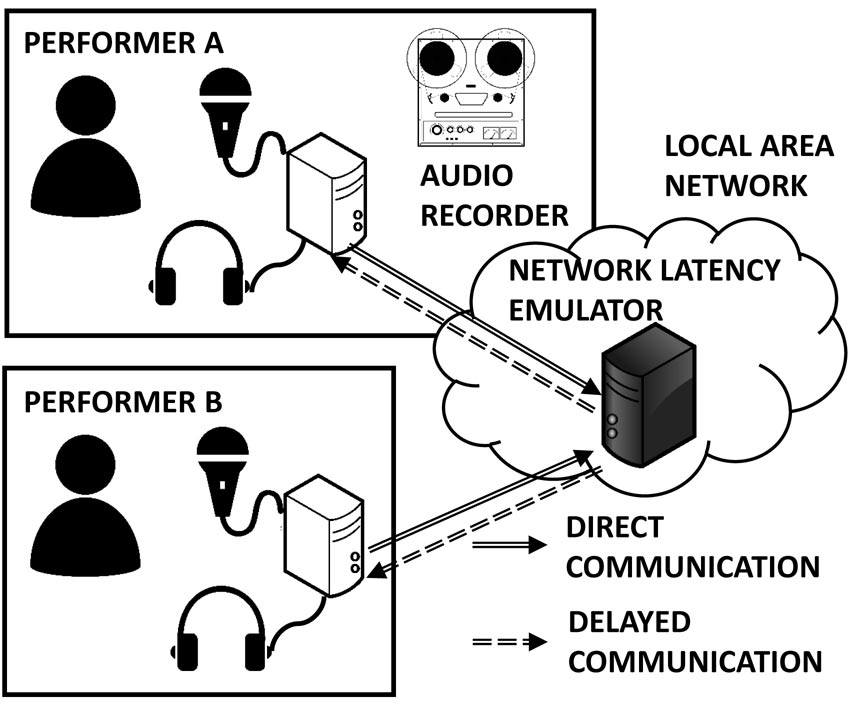
\includegraphics[width=.95\textwidth]{img/NMP/setup}
  \caption{Testbed setup}
 \label{fig:NMP:testbed}
\end{figure}
In order to analyze the correlation of the music played with the tolerance to delay, we implemented a testbed setup to emulate the NMP scenario. Our experiments involved pairs of musicians playing in two phono-insulated near-anechoic rooms (sound rooms), to avoid any audio feedback or visual contact, as depicted in Figure \ref{fig:NMP:testbed}. Visual contact was provided not even by means of video streaming because video processing time is larger than audio processing time and would have increased the minimum achievable end-to-end delay. The musicians were also forbidden to verbally communicate to their counterpart during the performance. Each room was equipped with a desktop PC running the SoundJack software, which is a peer-to-peer publicly available software \cite{carot2008distributed} that also implements a direct real-time evaluation of the experienced one-way end-to-end latency (thus including processing, buffering and playout delays).  Each PC was connected to an external sound card via high-speed connection (FireWire and AES/EBU) operating at a sampling rate of 48 kHz. The sound card was connected to high-quality headphones and microphones. An additional PC (with two network interfaces) running the WANem network emulator \cite{wanem} was placed in between. 
Through the WANem emulator we could manually select the delay and jitter of the emulated network, in order to replicate the NMP real-world scenario. The network interfaces of the three PCs were connected to each other through a Fast Ethernet switch. The PCs of the sound rooms were configured to communicate exclusively through the interfaces of the WANem emulator, thus preventing any direct communication between them. 

Each musician was able to hear their own instrument as well as the instrument of the other player through headphones. The choice of the headphones was made in order to minimize the possible delay and to avoid loop-feedback effects. The two audio signals were transmitted through the Local Area Network of the building. During the experiments, all the involved LAN segments were free of other traffic. The audio tracks were recorded as follows: the audio data generated by \textit{performer A} were recorded directly after the electric transduction of the microphone, whereas the audio data generated by \textit{performer B} were recorded from the SoundJack feedback after propagation of the audio stream through the network, i.e. as heard through \textit{performer A}'s headsets.

%\subsection{Scores and Network Parameters}
We considered three different music pieces: \textit{Yellow Submarine} (by The Beatles) at different values of BPM (88,110,132), \textit{Bolero} (by Maurice Ravel), and \textit{Master Blaster} (by Stevie Wonder), arranged for four different parts: main melody (M), chord comping (CC), sustained harmony (SH), and drums (D).  Scores were released to the musicians in advance.

\begin{table}[tb]
  \caption{Combination of parts played in each experiment session. M: main melody; CC: chord comping; SH: sustained harmony; D: drums}
  \centering %\small
  \label{tab:NMP:sessions}
  \bgroup
  \def\arraystretch{1.5}
 \begin{tabular}{||c|c|c|c|c||}
 \hline
 \hline
  Id & Instrument A& Part A & Instrument B & Part B \\
 \hline
 \hline
  1 & Acoustic Guitar & M & Classic Guitar & CC\\
  2 & Electric Piano & M & Drums & D\\
  3 & Keyboard (strings)  & SH & Drums & D\\
  4 & Keyboard (strings)  & SH & Electric Guitar & CC\\
  5 & Clarinet & M & Clarinet & M\\
  6 & Electric Guitar  & CC & Drums & D\\
  7 & Keyboard (strings)  & SH & Clarinet & M\\
 \hline
 \hline
   \end{tabular}
   \egroup
\end{table}

Our experiments involved 8 musicians with at least 8 years of musical experience, all with semi-professional or professional training level, and 7 instruments, i.e.:
Acoustic, Classic and Electric Guitar, Clarinet, Drums, Electric Piano and Keyboards with strings samples. Each musician played at least one of the instruments. The musicians were grouped in 7 pairs according to the combinations listed in Table \ref{tab:NMP:sessions}. Note that some musicians performed in more than one pair (e.g., one clarinetist performed twice, i.e. in pairs 5 and 7, whereas the pianist played electric piano and keyboard in pairs 2, 3, 4 and 7). For a given pair, each musician performed only one of the four parts for each of the three considered musical pieces, as detailed in Table \ref{tab:NMP:sessions}. Musicians in pairs 5 and 6 had regularly performed together in the last years, where the remaining pairs had never played together before. However, in order to avoid biases due to prior common performances, all the pairs were allowed to practice together in the testbed environment until they felt sufficiently confident. Before participating to our experiments, none of the players had ever experienced networked music interactions.

\begin{table}[tb]
  \caption{Tested network parameters and tempo settings}
  \centering %\small
  \label{tab:NMP:param}  
  \bgroup
  \def\arraystretch{1.5}
  \begin{tabular}{||c|c|c|c||}
\hline
\hline
 Piece & $\delta$ [BPM]& $\mu$ [ms]& $\sigma$ [ms]\\
\hline
\hline
 Yellow Submarine & 88,110,132 & 20,30,40,50,60 & 1 \\
 Bolero & 68  & 20,30,40,50,60 & 1 \\
 Master Blaster & 132  & 20,30,40,50,60 & 1 \\
\hline
\hline
  \end{tabular}
  \egroup
\end{table}

The recording procedure was repeated several times for each piece. As reported in Table \ref{tab:NMP:param}, each recording was characterized by different tempi and network settings in terms of reference BPM ($\delta$), network latency and jitter. The two latter parameters were set by assigning each IP packet a random delay $T_{net}$, statistically characterized by independent identically distributed Gaussian random variables with mean $\mu$ and standard deviation $\sigma$. The payload of each packet contained $128$ 16-bit-long audio samples, corresponding to a duration of $2.67$ ms. For the considered values of $\mu$ and $\sigma$, we set the receiver buffer size to 4 packets (i.e. $512$ audio samples) and measured the number of buffer overruns/underruns during each recording. The overall probability of overrun/underrun events turned out to be smaller than $1\%$. This value is representative of realistic traffic conditions of a telecommunication network. Note that overruns/underruns generate glitches (i.e., distortions in the reproduction of the received audio signal) which affect the overall audio quality perceived by the musicians. 
 

Note also that, as $T_{net}$ accounts only for the emulated network delay, the additional latency $T_{proc}$ introduced by the audio acquisition and the audio rendering processes must be taken into account in the computation of the one-way overall delay time $T_{tot}=T_{net}+ T_{proc}$.
More specifically, the processing time $T_{proc}$ includes: in-air sound propagation from instrument to microphone; transduction from the acoustic wave to electric signal in the microphone; signal transmission through the microphone's wire; analog to digital conversion of the sender's sound card, internal data buffering of the sound card; processing time of the sender's PC to packetize the audio data prior to transmission; processing time of the receiver's PC to depacketize the received audio data; queuing time of the audio data in the application buffer at the receiver side; digital to analog conversion of the receiver's sound card; transmission of the signal through the headphone's electric wire; transduction from electric signal to acoustic wave in the headphones.
We experimentally evaluated $T_{proc}$ by measuring the end-to-end delay $T_{tot}$ when setting $\mu=0$ and $\sigma=0$, i.e., $T_{net}=0$. Given the setup in Figure \ref{fig:NMP:testbed}, we substituted the headphones with a loudspeaker and placed the microphone a few centimeters away from the speaker, in the room of the Performer B (room B). We then generated a synthetic click in the room A that was recorded by the audio recorder and, at the same time, it was transmitted to room B. In room B, the click was executed by the speaker, captured by the microphone and fed back to the audio recorder, where it was recorded again. By estimating the time lag between the recordings of the two clicks, we obtain the double of the end-to-end delay. The measured time was $T_{proc}=15$ ms, which is larger than the one reported in \cite{carot2007networked}. This is mainly due to the use of generic sound card drivers, which increased the processing time of SoundJack. Please note the acoustic delay due to the distance between the speaker and the microphone in room B is about 30 microseconds for each centimeter of distance and can therefore be neglected in the final computation of $T_{proc}$.

During each recording session, the order of the proposed network configurations was randomly chosen and was kept undisclosed to the testers, in order to avoid biasing or conditioning. Two measures of metronome beats at the reference BPM were played before the beginning of each performance. In order to consider a lower number of variables, we asked the participants to strictly follow the assigned tempo and therefore to avoid the deviations of the tempo which typically occur during an expressive performance. At the end of each performance, the testers were asked to express a rating on the quality of their interactive performance. The details on such quality are provided in the next Section.

%\subsection{Collection of the signal domain and the semantic codomain}\label{sec:NMP:domain}
%We formalize the signal domain by extracting rhythmic and timbral features from the recordings of the performance and from the score of the parts. The quality of performances is evaluated by means of subjective metrics, asked to the musicians after each performance, and of objective metrics, through a processing technique from the recordings.


\subsection{The feature representation of the signal domain}\label{sec:NMP:domain}

\begin{table}[tb]
  \caption{Timbral characterization for each instrument}
  \centering %\small
  \label{tab:NMP:instruments}
  \bgroup
  \def\arraystretch{1.5}
\begin{tabular}{||c|c|c|c|c|c|c||}
 \hline
 \hline
 Instrument  & $SC$ & $SSp$ & $SSk$ & $SK$ & $SF$ & $SE$ \\
 \hline
 \hline
Ac. Guitar &   2047 & 4109 & 2.76 & 10.25 & 0.19 & 0.76 \\
Clarinet & 1686 & 2272 & 4.85 & 31.81 & 0.07 & 0.731 \\
Cl. Guitar &   3263 & 4680 & 1.57 & 4.43 & 0.22 & 0.841 \\
Drums & 7903 & 7289 & 0.35 & 1.57 & 0.61 & 0.936 \\
El. Guitar & 1848 & 2522 & 3.70 & 23.46 & 0.09 & 0.818 \\
El. Piano & 2101 & 4251 & 3.16 & 12.26 & 0.16 & 0.734 \\
Keyboard & 1655 & 3065 & 4.39 & 23.77 & 0.1 & 0.733 \\
 \hline
 \hline
   \end{tabular}
   \egroup
\end{table}

We formalize the signal domain by extracting timbral and rhythmic descriptors from the recordings of the performance and from the score or symbolic representation of the parts, respectively. 

With respect to the timbral features, we consider the timbre as a property of the instruments. We aim to investigate how the sound quality affects the musicians' tolerance to the network delay, by making the assumption that the networked delay does not affect the timbral descriptors. For this reason, we do not track the evolution of the timbre during the performances and we asked the musicians to play with a flat dynamics during the performance, in order to reduce the possible oscillations of the timbral descriptors. For each instrument, we compose an audio file with a representative selection of recordings of its timbre. We take into consideration a variety of pitches from the musical range of the instrument, so to include possibly different registers of the same instrument. For example, the timbral characterization of the drums included the recording of each percussive instrument from the drum set, whereas the characterization of guitar included different kinds of playing techniques, like chords played as arpeggio and plucked strings. 


\begin{figure}[!tb]
		\subfloat[Different values of $SC$]{\includegraphics[width=.47\textwidth]{img/NMP/value_SC}\label{fig:NMP:value_SC}}  \hfil
		\subfloat[Different values of $SSp$]{\includegraphics[width=.47\textwidth]{img/NMP/value_SSp}\label{fig:NMP:value_Ssp}}  \hfil
		\subfloat[Different values of $SSk$]{\includegraphics[width=.47\textwidth]{img/NMP/value_SSk}\label{fig:NMP:value_SSk}}  \hfil
\subfloat[Different values of $SK$]{\includegraphics[width=.47\textwidth]{img/NMP/value_SK}\label{fig:NMP:value_SK}}  \hfil
		\subfloat[Different values of $SF$]{\includegraphics[width=.47\textwidth]{img/NMP/value_SF}\label{fig:NMP:value_SF}}  \hfil
\subfloat[Different values of $SE$]{\includegraphics[width=.47\textwidth]{img/NMP/value_SE}\label{fig:NMP:value_SE}}  \hfil
	\caption{Values of spectral descriptors for the different instruments}
	\label{fig:NMP:values_spec}
\end{figure}

From the representative audio files we then extract the following features: Spectral Centroid ($SC$), Spectral Spreadness ($SSp$), Spectral Skewness ($SSk$), Spectral Kurtosis ($SK$), Spectral Flatness ($SF$) and Spectral Entropy ($SE$). The definition and interpretation of such features is provided in the Section \ref{app:LLFs} and summarized in Table \ref{tab:LLFs:features}. It is worth remembering that the Spectral Centroid provides an indicator of the brightness of the timbre, while Spectral Entropy and Flatness can be interpreted as an estimate of the noisiness. 

The spectral features are extracted by means of the MIRToolbox \cite{Lartillot2007} from a frame-based representation of the audio files, and their average values over the frames are computed. Since we consider a selection of different pitches and playing techniques, the obtained values reported in Table \ref{tab:NMP:instruments} and Figure \ref{fig:NMP:values_spec} can be seen as an overall indicator of the instrument's timbral properties. We can notice that the Drums exhibit the highest values of Flatness and Entropy, hence noisiness, and a rather high Spectral Centroid. On the other side, the Clarinet presents the lowest value of noisiness and a low Spectral Centroid, given by its rather harmonic timbre. Among the guitars, we do not use distortion effect for the Electric Guitar, hence its timbre is rather clean and has a lower Spectral Flatness than the Acoustic Guitar, while showing a higher Entropy.

\begin{table}[tb]
  \caption{Rhythmic characterization of the musical pieces performed during the tests}
  \centering %\small
  \label{tab:NMP:pieces}  
  \bgroup
  \def\arraystretch{1.5}
 \begin{tabular}{||c|c|p{1.4cm}|p{1.4cm}|p{1.8cm}|p{1.8cm}|p{1.8cm}||}
 \hline
 \hline
Part &  Feature & Bolero & Master Blaster & Yellow Submarine (88 BPM) & Yellow Submarine (110 BPM) & Yellow Submarine (132 BPM)\\
 \hline
 \hline
 \multirow{2}{*}{M}& $ED$ & 2.1407 & 2.1667 & 1.5253 & 1.9067 & 2.2880 \\
           & $RC$ & 5.5337 & 5.5627 & 5.4160 & 5.7094 & 6.0567 \\
\hline
\multirow{2}{*}{CC}& $ED$ & 1.3222 & 2.6542 & 1.8333 & 2.2917 & 2.7500 \\
          & $RC$ & 3.4516 & 6.8903 & 5.3064 & 5.6455 & 5.9592\\
\hline
\multirow{2}{*}{SH}& $ED$ & 0.3778 & 0.5778 & 0.8213 & 1.0267 & 1.2320 \\
          & $RC$ & 2.9364 & 5.3444 & 3.8062 & 4.0208 & 4.2237\\
\hline
\multirow{2}{*}{D}& $ED$ & 2.0148 & 4.3514 & 1.5253 & 1.9067 & 2.2880 \\
         & $RC$ & 6.0285 & 5.7255 & 4.5228 & 4.7548 &  4.9767 \\
 \hline
 \hline
   \end{tabular}
   \egroup
\end{table}



With respect to the rhythmic features, we extract the MLFs described in Section \ref{sec:LLFs:hand-crafted}, i.e., the Rhythmic Complexity ($RC$) and the Event Density ($ED$). As mentioned, the tempo was fixed and provided to the musician, and a particular song, \textit{Yellow Submarine}, was executed at different tempi. We manually compute the Event Density \cite{Lartillot2007} from the sheet music of the parts and we extract the Rhythmic Complexity \cite{povel} using the MIDI Toolbox \cite{Eerola2004}. The Rhythmic Complexity is a weighted sum of different metrics computed from the distribution and position of the onsets in the sheet music. The mathematical definition and the weights used in \cite{Eerola2004} are discussed in Section \ref{app:LLFs}. 

The rhythmic features for each part are summarized in Table 
\ref{tab:NMP:pieces} and shown in Figure \ref{fig:NMP:values_rhythm}. We notice that the Sustained Harmony has generally low values of Event Density and Rhythmic Complexity, since it usually involves one onset every measure. On the other side, the Chord Comping of \textit{Master Blaster} and the drums in \textit{Bolero} are rhythmically challenging, due to the variation between even and odd patterns. Moreover, since the Event Density depends on the tempo and Rhythmic Complexity depends on Event Density, we notice that increasing the BPM of \textit{Yellow Submarine} produces an increase of both features.


\begin{figure}[!tb]
	\subfloat[Different values of $ED$]{\includegraphics[width=.47\textwidth]{img/NMP/value_ED}\label{fig:NMP:value_ED}}  \hfil
	\subfloat[Different values of $RC$]{\includegraphics[width=.47\textwidth]{img/NMP/value_RC}\label{fig:NMP:value_RC}}  \hfil
	
	\caption{Values of rhythmic descriptors for the different combination of parts/songs}
	\label{fig:NMP:values_rhythm}
\end{figure}



%in this study we provide an evaluation of the impact of network conditions on the quality of the musical experience, according to the type of the instruments and to some characteristics of the performance. As far as the type of instrument is concerned we adopt a timbral feature-based representation, whereas we exploit musical part, Event Density \cite{Lartillot2007} and Rhythmic Complexity \cite{povel} of the performed pieces to characterize the performance. 

\subsection{The quality metrics}\label{sec:NMP:codomain}
Several perceptual and musicological aspects affect the perception of the overall quality of a performance and therefore it is not clear how to measure such quality. Musicians are the ideal candidates to estimate it, since they usually evaluate their own performance, during rehearsals, in order to improve their skills. For this reason, we define two subjective metrics annotated directly by the musicians involved in the performance. Such subjective metrics are however affected by the personal bias of the musicians: two musicians might differently rate the overall quality of the same performance, according to their experience or the importance they assign to different aspects. In order to ease these subjectivity issues, we also define an objective metric, which is unbiased from the musicians' opinion, by computing the trend of the tempo over the performance.

At the end of each of the recordings, we asked the musicians to rate the quality of the performance. The musicians provided two annotations: one about the quality of the interaction and one about the perception of the delay. The former is defined as the perceived quality $Q_{perc}$, and is annotated within a five-valued range, from $Q_{perc}=1$, meaning the performance was very poor, to $Q_{perc}=5$, i.e., very good. The metric $Q_{perc}$ is not related to the audio quality experienced by the musicians, but only to the evaluation of the overall satisfaction of their experience and interaction with the counterpart. The latter is defined as the perceived network delay, $D_{perc}$, and it ranges between $1$, i.e., the delay was intolerable, and $4$, i.e., the delay was not perceivable. The value $D_{perc}=3$ indicates a slightly perceivable delay, and the value $D_{perc}=2$ indicates a more perceivable delay, but still tolerable for the sake of the performance. The choice of the values of $D_{perc}$ was made to help the players in the annotation task, since it is more common to use evaluation scales where the positive values are the higher values and vice-versa. In case the players spontaneously aborted their performance within the first $50$ seconds, $D_{perc}$ was set to $1$ and $Q_{perc}$ was set to $0$ by default. 

After the recording sessions, we extract the objective quality metric as the trend of the tempo during the performances, i.e., the tendency to slow down or accelerate in the initial part of the performance. For the first $50$ seconds we compute a linear regression of the BPM over the sparse BPM measurements. In order to do so, we first manually annotate the beats of the performance, as it is indicated in the music score. We estimate the beats occurring in the silences as equally distant from the surrounding beats. We are able to compute the instantaneous BPM from the time difference between two consecutive beats. We compute the BPM trend by smoothing the sequence of instantaneous BPM. The audio tracks are divided in $N=20$ time windows, each lasting $5$~s, with a 50\% overlap ($2.5$~s). For each time window, we compute the average BPM as $b(t_n)$ with $t_n=n\cdot 2.5$s and $n=1,...,N$. We estimate the tendency of the performance to accelerate or decelerate by considering the slope of the linear approximation of the BPM trend. We estimate the intercept $\beta$ and the slope $\kappa$ with linear interpolation, 
\begin{equation}
\argmin{\kappa, \beta} \frac{1}{N} \sum_{n=1}^{N} \left(b(t_n)-(\kappa t_n + \beta)\right)^2.
\end{equation}
In our experiments, the average Mean Square Error of the linear approximation is about $1.75$\%, i.e., it is accurate to approximate the BPM trend as a first order polynomial.

We consider the slope $\kappa$ as the objective metric for the evaluation of the performance quality: $\kappa=0$ means steady tempo; $\kappa>0$ means that the musician is accelerating; $\kappa<0$ means that the musician is slowing down and thus is unable to keep up with the tempo. 
%
%\subsection{Numerical results}\label{sec:NMP:results}
%In this Section, we build the linking function by means of a manual data analysis. We first provide some general and qualitative considerations on the BPM trend of the performance, and then we discuss the quantitative analysis of the NMP.



\subsection{Qualitative evaluation}\label{sec:NMP:qualResults}

We first provide some qualitative comments on the trend of the BPM curve $b(t_n)$ extracted from the execution of \textit{ Yellow Submarine} for different combinations of instruments and parts, various values of $T_{tot}$ in the range between $15$ and $75$ ms and three different values of $\delta$ (as reported in Table \ref{tab:NMP:param}). The lower bound of the tested delay values (i.e. $T_{tot}=15$ ms) is obtained by setting $T_{net}=0$ ms, meaning that no network delay is added to the unavoidable processing time $T_{proc}$. For values of $T_{tot}$ above $75$ ms (i.e., when $T_{net}=60$ ms), a considerable amount of executions were aborted by the musicians due to the extreme difficulty in maintaining synchronization. Therefore, we limit our analysis to delay ranges which allowed every pair of musician to perform the piece uninterruptedly for at least one minute.
The results are reported in Figures \ref{fig:NMP:melody} and \ref{fig:NMP:drums}, while the legend is shown in Figure  \ref{fig:NMP:legend}. The different colors identify the amount of total network delay $T_{tot}$ applied, while the style of the lines identifies the nominal BPM. The results show that in almost all the considered recordings an initial deceleration occurs in the first few seconds, when the players adjust their tempo until they find a balance, allowing them to reach the required degree of synchronization. Such initial deceleration is nearly absent for small network end-to-end delays and reference BPM, but it becomes much more pronounced for large values of $T_{tot}$ and $\delta$. In particular, the scenario with $\delta=132$ BPM and $T_{tot}=75$ ms presents an initial tempo reduction of 12-20 BPM in all the tested combinations of instruments and parts.
In addition, as shown in Figure \ref{fig:NMP:melody}, combining typically non-homorhythmic parts such as Melody (M) and Chord Comping (CC) or M and Sustained Harmony (SH) leads either to a tendency to constantly decelerate (see Figure~\ref{fig:NMP:melody}, left-hand side), which is more pronounced for large $\delta$ , or to a \lq\lq saw tooth'' pattern in which the players periodically try to compensate the tempo reduction (Figure \ref{fig:NMP:melody}, middle). Note that, in the latter case, there is no such pattern in the benchmark scenarios with $T_{tot}=15$ ms. The difference in the behavior of SH and CC when interacting with M is also due to the type of rhythmic interplay that takes place. Chord Comping, in fact, tends to closely follow and match the tempo of the Melody, while Sustained Harmony is a steady accompaniment (``pad") with more relaxed on-time constraints. As M is expected to meander off-tempo, it is harder for SH and M to stay in sync, and adjustments happen in bursts.


\begin{figure}[!th]
	
		\subfloat[Combinations for the Melody part with the Chord Comping and the Sustained Harmony parts, and between the Chord Comping and the Sustained Harmony parts] {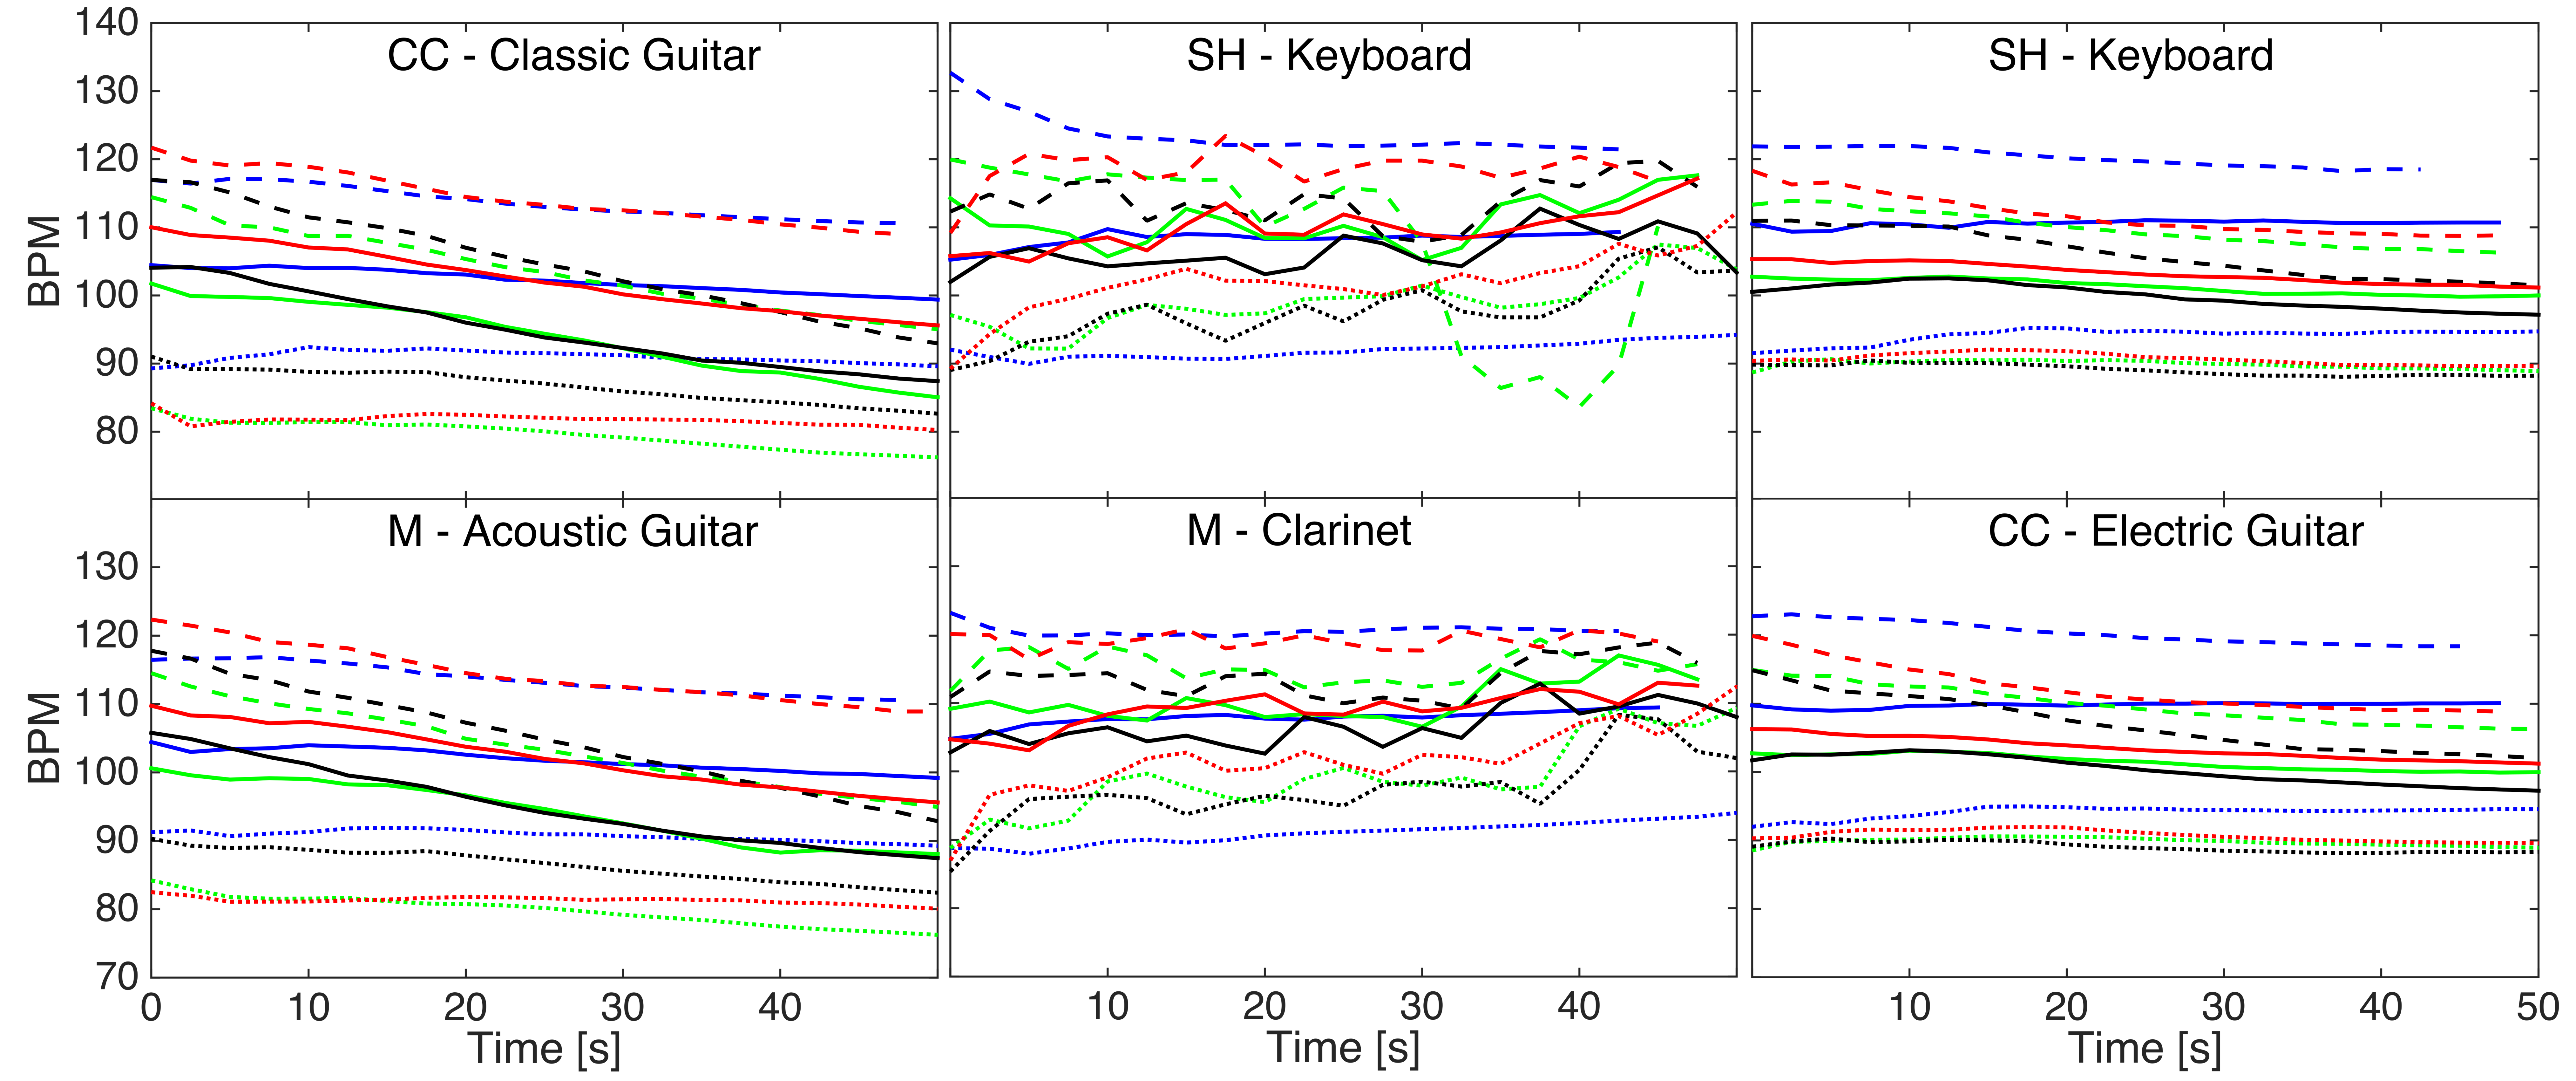
\includegraphics[width=\textwidth]{img/NMP/fig1_wider}\label{fig:NMP:melody}}  
		\hfil
		\subfloat[Combinations for the Drum part with the Chord Comping, the Sustained Harmony and the Melody parts]{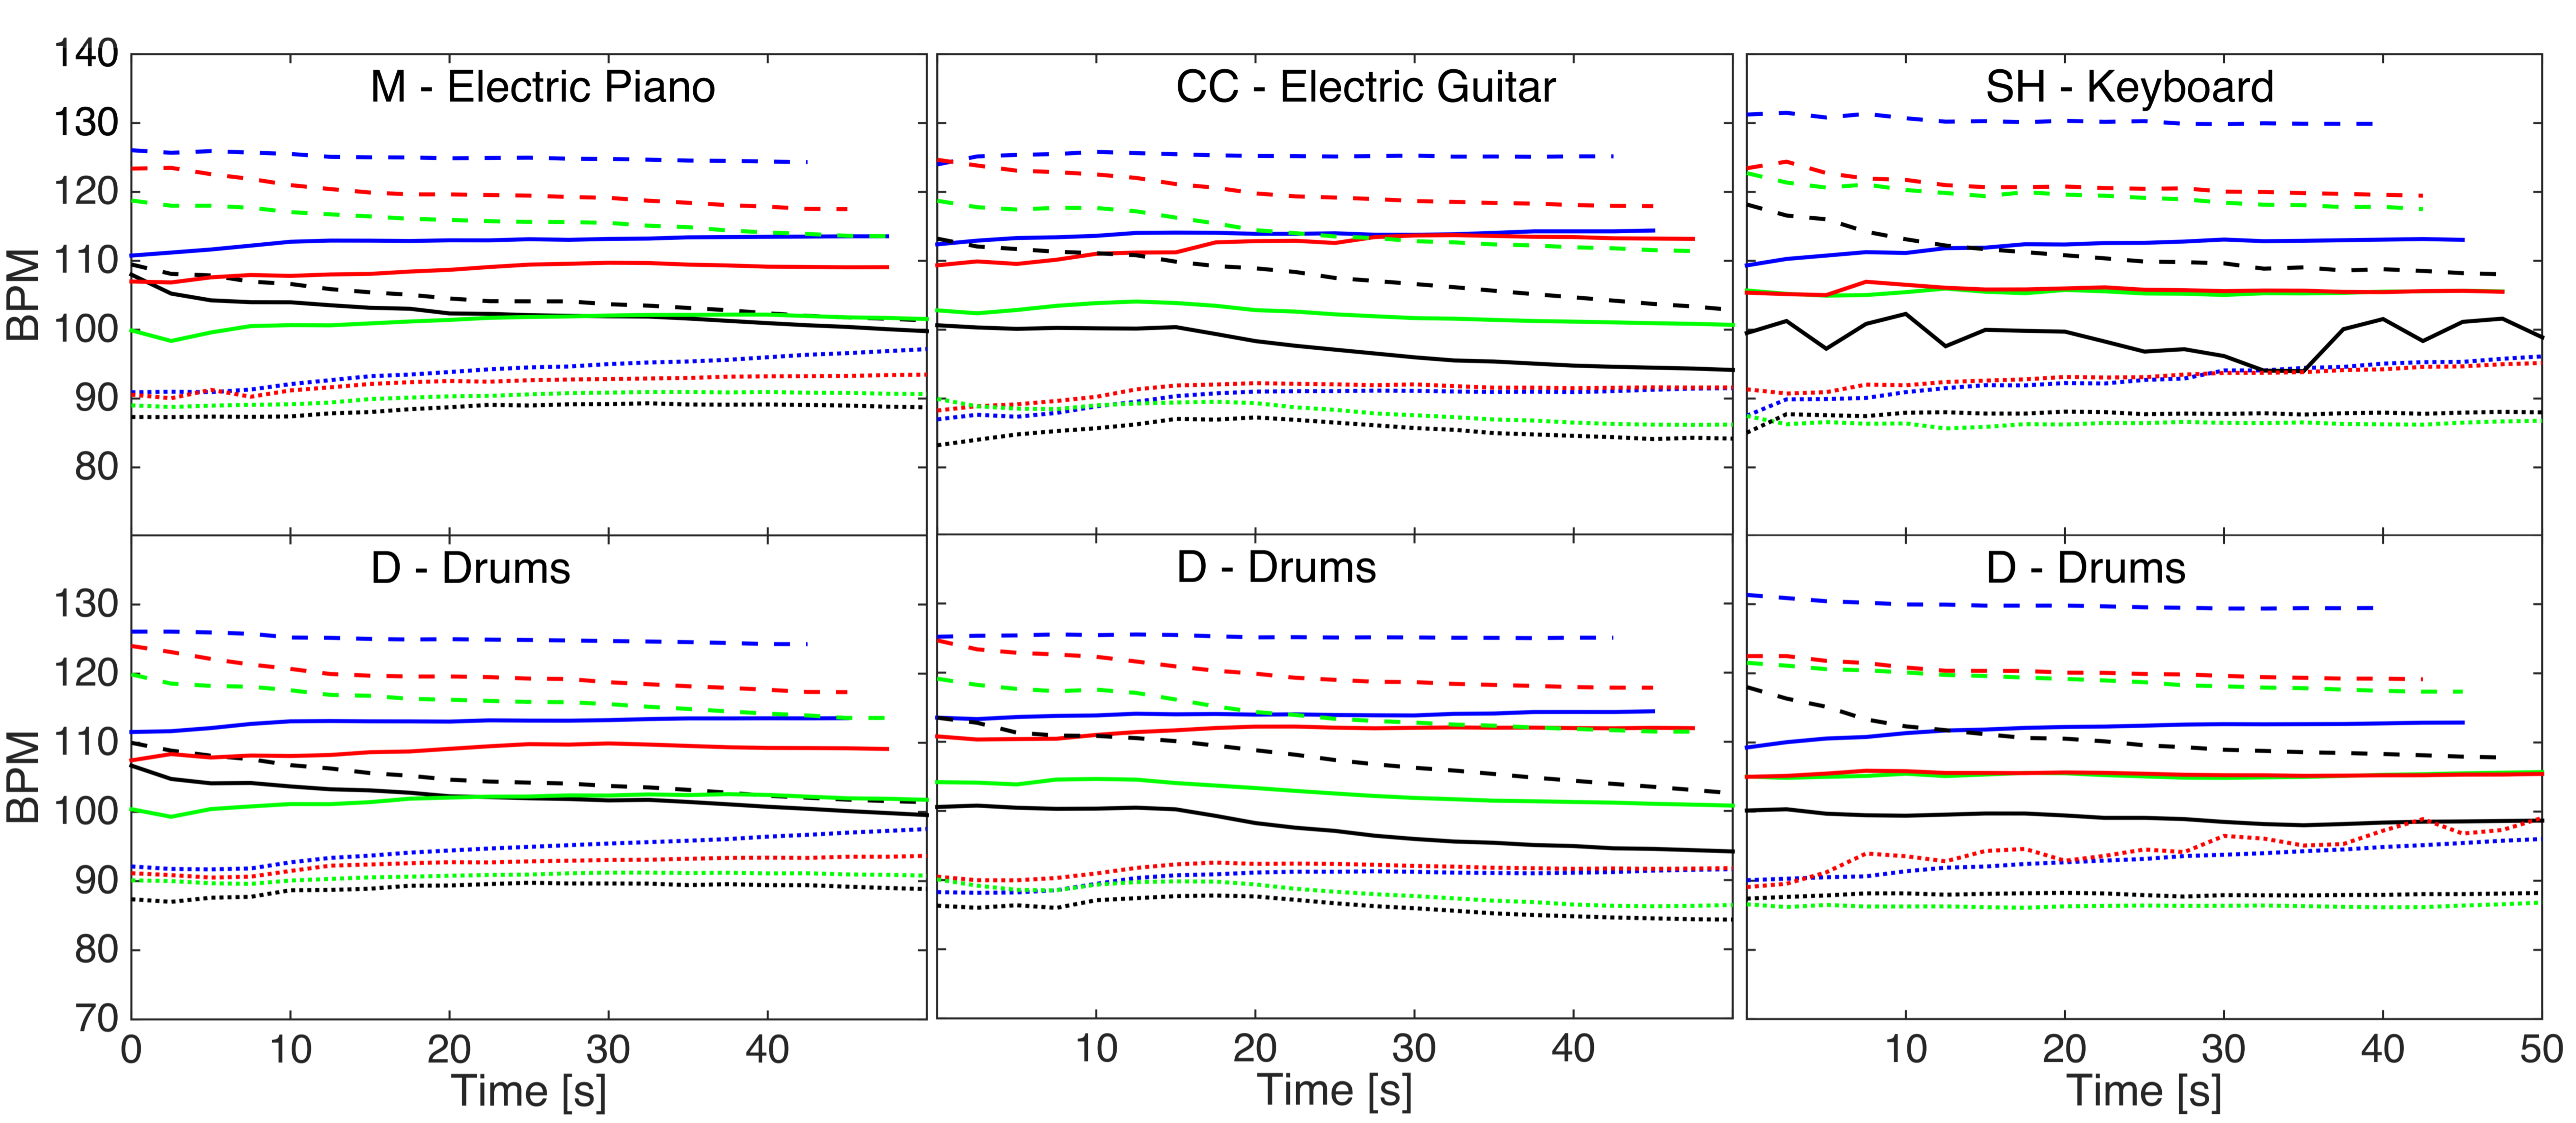
\includegraphics[width=\textwidth]{img/NMP/fig2_wider}\label{fig:NMP:drums}}%\centering
\caption{BPM trend over time when playing \textit{Yellow Submarine}, for different combinations of parts, instruments, end-to-end delays $T_{tot}$ (identified by the color) and reference BPMs $\delta$, identified by the type of line (solid, dashed, dotted). }
\label{fig:NMP:qualTot}
\end{figure}

\begin{figure}[!th]
	\centering
	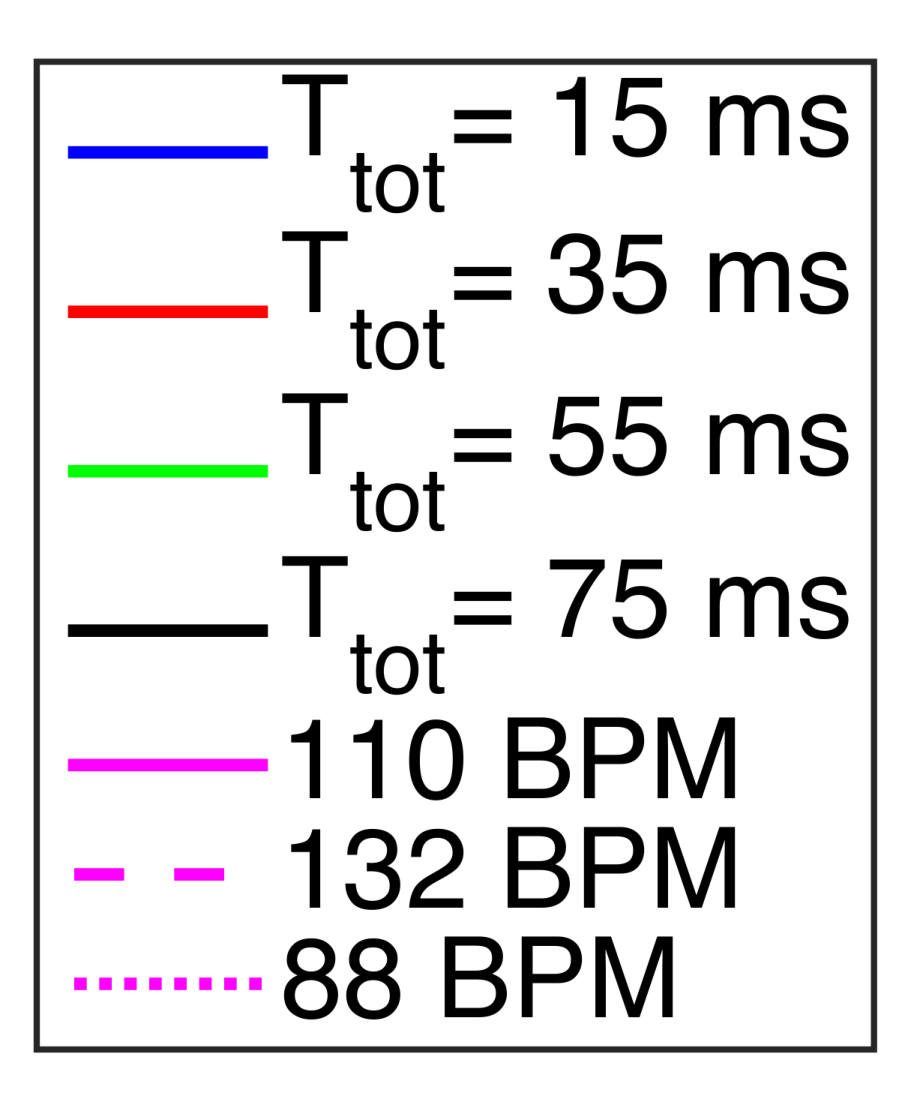
\includegraphics[width=0.2\textwidth]{img/NMP/legend_smaller}
	\caption{Legend for Figures \ref{fig:NMP:melody} and \ref{fig:NMP:drums} }
	\label{fig:NMP:legend} 
\end{figure}


When two homo-rhythmic parts (those that are expected to keep a steady tempo, such as CC and SH) are combined, $b(t_n)$ tends to remain almost constant (see Figure \ref{fig:NMP:melody}, on the right-hand side, where a slight negative slope occurs only at $\delta=132$ BPM).
A similar behavior is observed when M, CC or SH combine with Drums (See Figure \ref{fig:NMP:drums}), despite the fact that the two parts are not always homo-rhythmic. This is due to the fact that drums tend to have a very specific rhythmic ``leading role" in western music, therefore the other musicians generally tend to follow the drummer.

Based on the above results, we conclude that the choice of the combination of instruments and parts has a significant impact on the capability of the musicians to keep a steady tempo. 
In the next Section, we will give a more in-depth analysis of the impact of single rhythmic and timbral features characterizing the specific combination of parts and instruments on the subjective and objective performance quality metrics.

\subsection{Quantitative evaluation}\label{sec:NMP:quantResults}
We now analyze the impact of different end-to-end delays $T_{tot}$ on the subjective quality metric $D_{perc}$ and on the BPM slope $\kappa$, for various values of the rhythmic and timbral features described in Section \ref{sec:NMP:domain}. The interaction quality rating $Q_{perc}$ resulted to be strongly correlated to $D_{perc}$, therefore for the sake of brevity we do not report such results.


%\subsubsection{Dependency of Quality Metrics on Rhythmic Features}
\begin{figure}[!tb]
\begin{flushright}
  \subfloat[Subjective Perception of Delay $D_{perc}$]{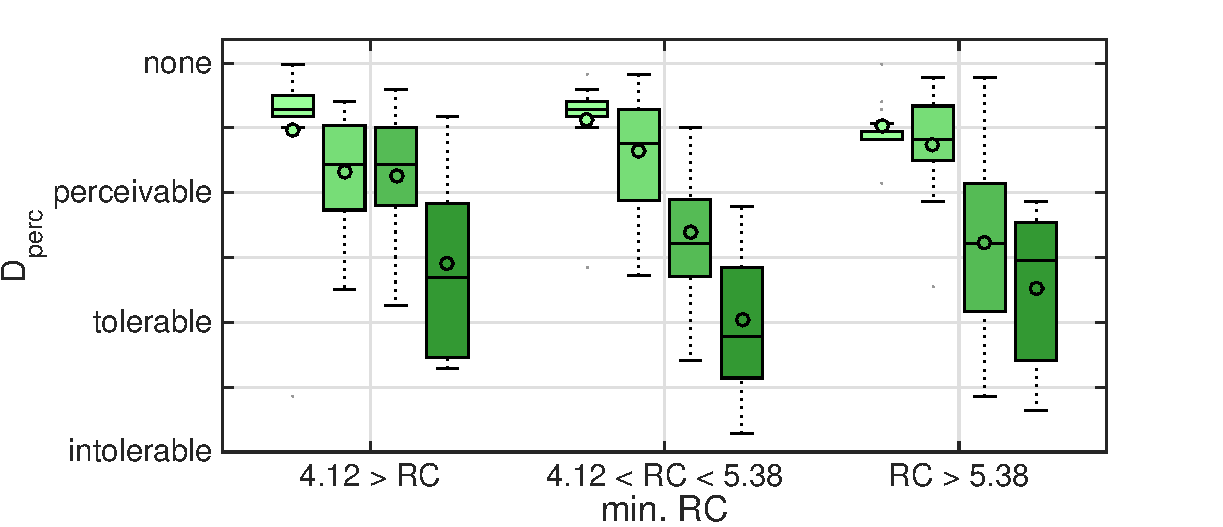
\includegraphics[width=.77\textwidth]{img/NMP/minRC_PD}\label{fig:NMP:minRC_SubjPerc}}  \hfil
  \subfloat[Average BPM Linear Slope $\kappa$]{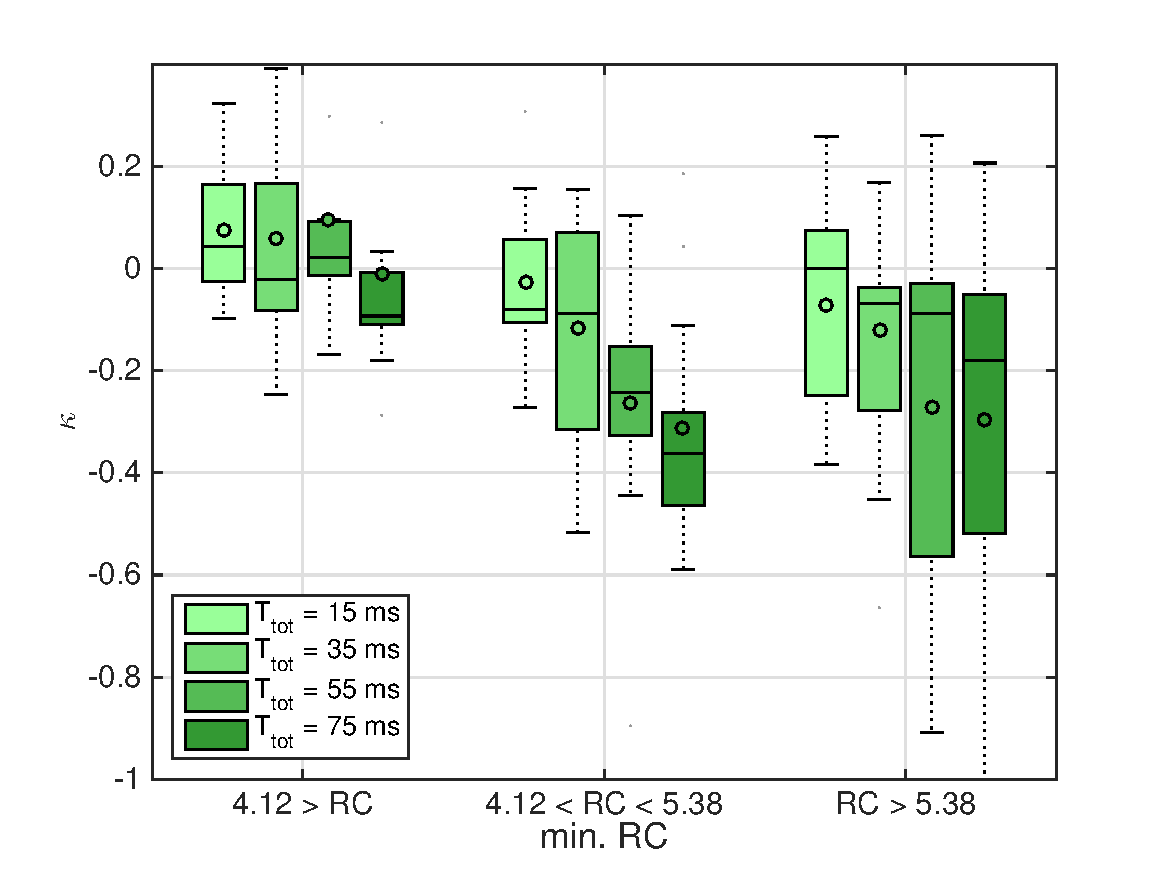
\includegraphics[width=.72\textwidth]{img/NMP/minRC_BPM}\label{fig:NMP:minRC_LinSlope}}        
\end{flushright}
\caption{Dependence of $\kappa$ and $D_{perc}$ on the minimum Rhythmic Complexity $RC$ for different values of $T_{tot}$.}
\label{fig:NMP:minRC}
\end{figure}


 

For every recording, we consider the maximum and minimum values of each feature among the two parts and instruments played by the musicians. For example, in test session 2 (see Table \ref{tab:NMP:sessions}) when performing \textit{Bolero}, the minimum Event Density ($ED$) is 2.01 ($ED$ of the D part) and the maximum $ED$ is 2.14 ($ED$ of the M part). Conversely, the minimum Rhythmic Complexity ($RC$) is 5.53 (on the M part) and the maximum $RC$ is 6.03 (on the D part).

\begin{figure}[!tb]
\begin{flushright}
  \subfloat[Subjective Perception of Delay $D_{perc}$]{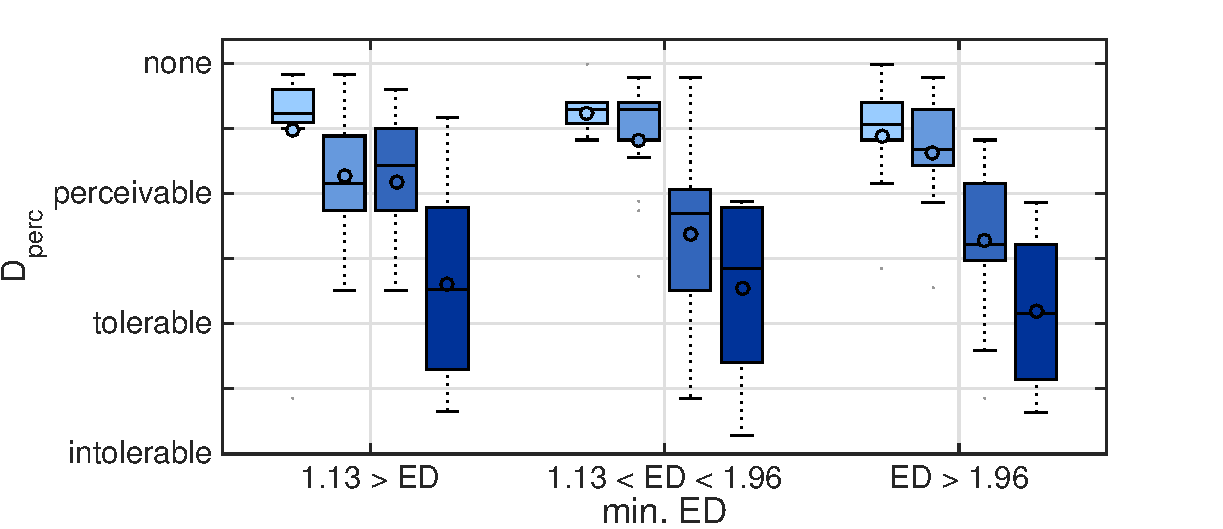
\includegraphics[width=.77\textwidth]{img/NMP/minED_PD}\label{fig:NMP:minED_SubjPerc}}  \hfil
  \subfloat[Average BPM Linear Slope $\kappa$]{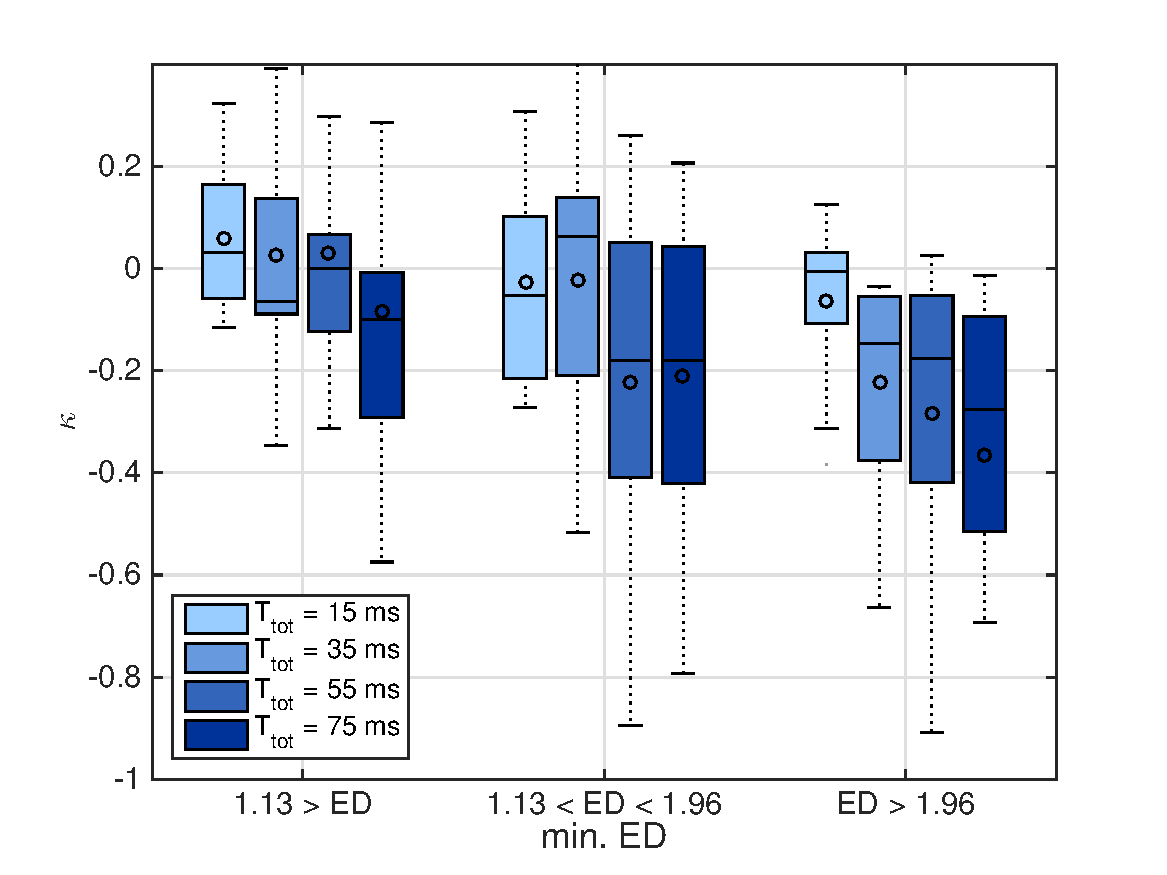
\includegraphics[width=.72\textwidth]{img/NMP/minED_BPM}\label{fig:NMP:minED_LinSlope}}        
\end{flushright}
\caption{Dependence of $\kappa$ and $D_{perc}$ on the minimum Event Density $ED$ for different values of $T_{tot}$}
\label{fig:NMP:minED}
\end{figure}

Figure \ref{fig:NMP:minRC_SubjPerc} reports the subjective delay perception $D_{perc}$ attributed by the pairs of testers to their performances, for different values of $T_{tot}$, as a function of the minimum $RC$ between the two parts. For the sake of clarity, only four values of $T_{tot}$ are reported, where $T_{tot}=T_{proc}=15$ ms is considered as benchmark. 

\begin{figure}[!tb]
\begin{flushright}
  \subfloat[Subjective Perception of Delay $D_{perc}$]{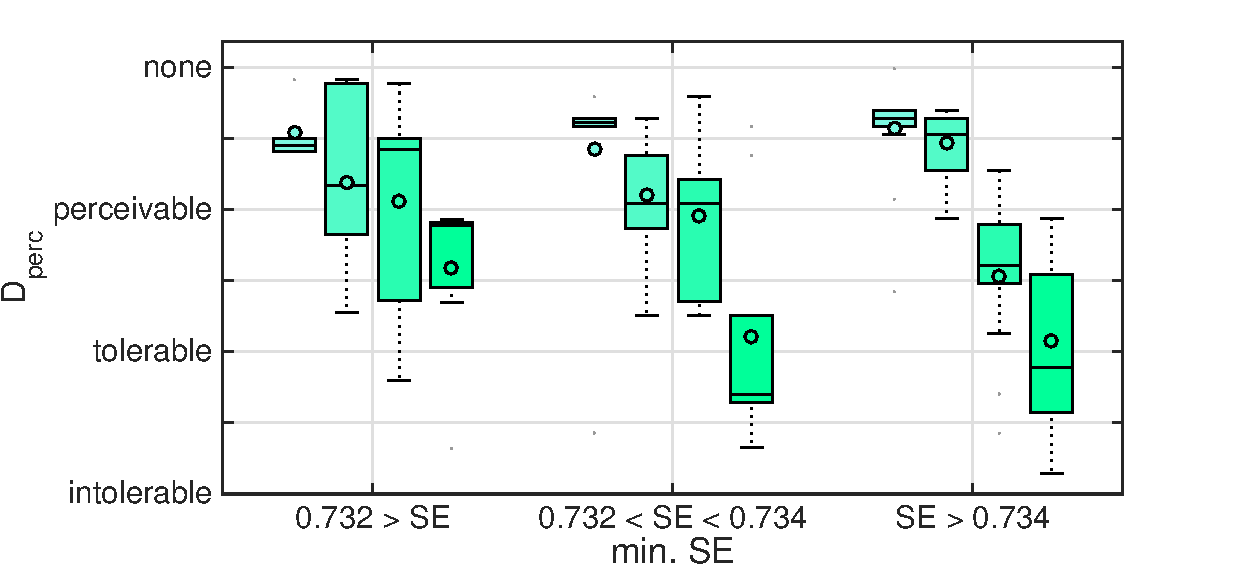
\includegraphics[width=.77\textwidth]{img/NMP/minSE_PD}\label{fig:NMP:minSE_SubjPerc}}  \hfil
  \subfloat[Average BPM Linear Slope $\kappa$]{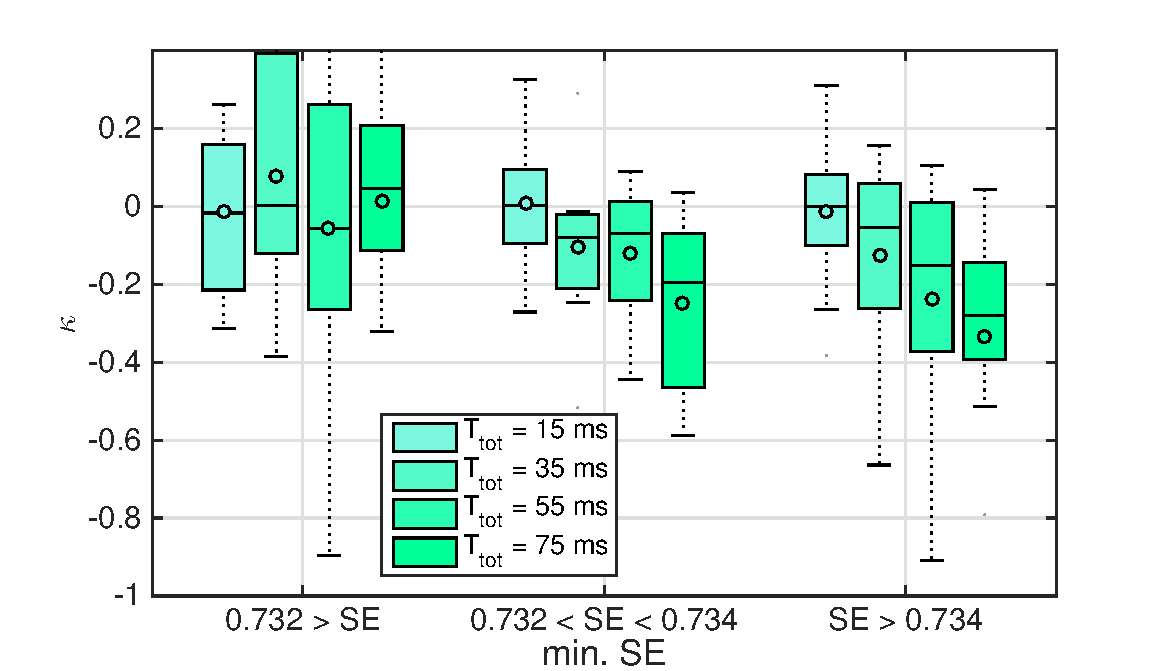
\includegraphics[width=.72\textwidth]{img/NMP/minSE_BPM}\label{fig:NMP:minSE_LinSlope}}        
\end{flushright}
\caption{Dependence of $\kappa$ and $D_{perc}$ on the minimum Spectral Entropy $SE$ for different values of $T_{tot}$}
\label{fig:NMP:minSE}
\end{figure}


Results show that, for a given value of minimum $RC$, the average $D_{perc}$ decreases when $T_{tot}$ increases. Moreover, for a given $T_{tot}$, increasing $RC$ also has a negative impact on the average quality rating. However, the reduction of $D_{perc}$ is more enhanced for large values of $T_{tot}$. 
%Similar results are obtained when considering the subjective delay perception $D_{perc}$, averaged over the pair of performers (see Figure \ref{}).

\begin{figure}[!tb]
\begin{flushright}
  \subfloat[Subjective Perception of Delay $D_{perc}$]{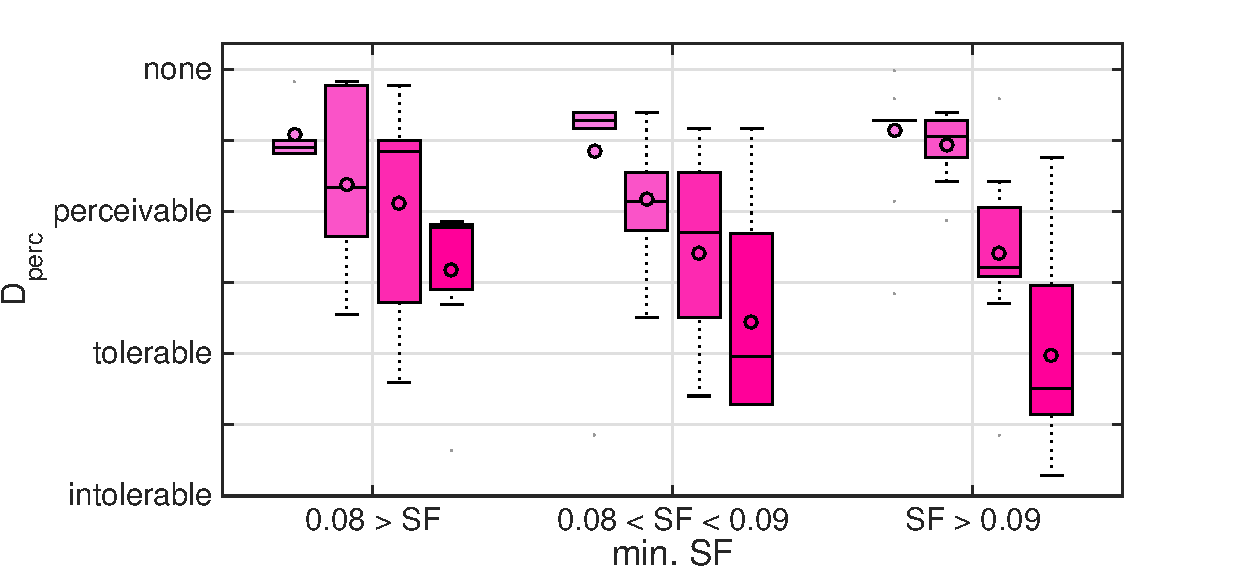
\includegraphics[width=.77\textwidth]{img/NMP/minSF_PD}\label{fig:NMP:minSF_SubjPerc}}  \hfil
  \subfloat[Average BPM Linear Slope $\kappa$]{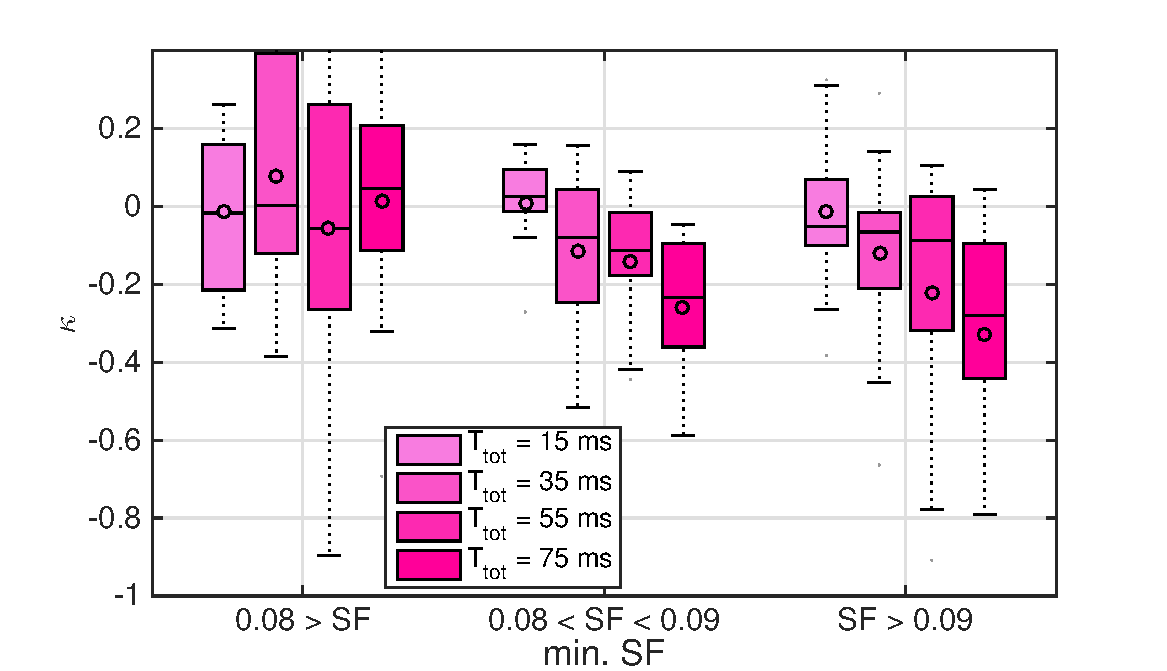
\includegraphics[width=.72\textwidth]{img/NMP/minSF_BPM}\label{fig:NMP:minSF_LinSlope}}        
\end{flushright}
\caption{Dependence of $\kappa$ and $D_{perc}$ on the minimum Spectral Flatness $SF$ for different values of $T_{tot}$}
\label{fig:NMP:minSF}
\end{figure}

We now analyze how the average BPM linear slope $\kappa$ is affected by the minimum rhythmic complexity $RC$. For large values of $RC$ (see Figure \ref{fig:NMP:minRC_LinSlope}), we found slightly negative values of $\kappa$ (which denote a tendency to slow down) even in the benchmark scenario. As expected, the need of synchronism increases when musicians are playing more complex parts and the lack of typical synchronization cues, such as eye-contact, affects the performance even in absence of network delay. However, negative slopes tend to become much steeper for large values of $T_{tot}$, which suggests that the tolerance to the delay decreases for more complex musical pieces.

\begin{figure}[!tb]
\begin{flushright}
  \subfloat[Subjective Perception of Delay $D_{perc}$]{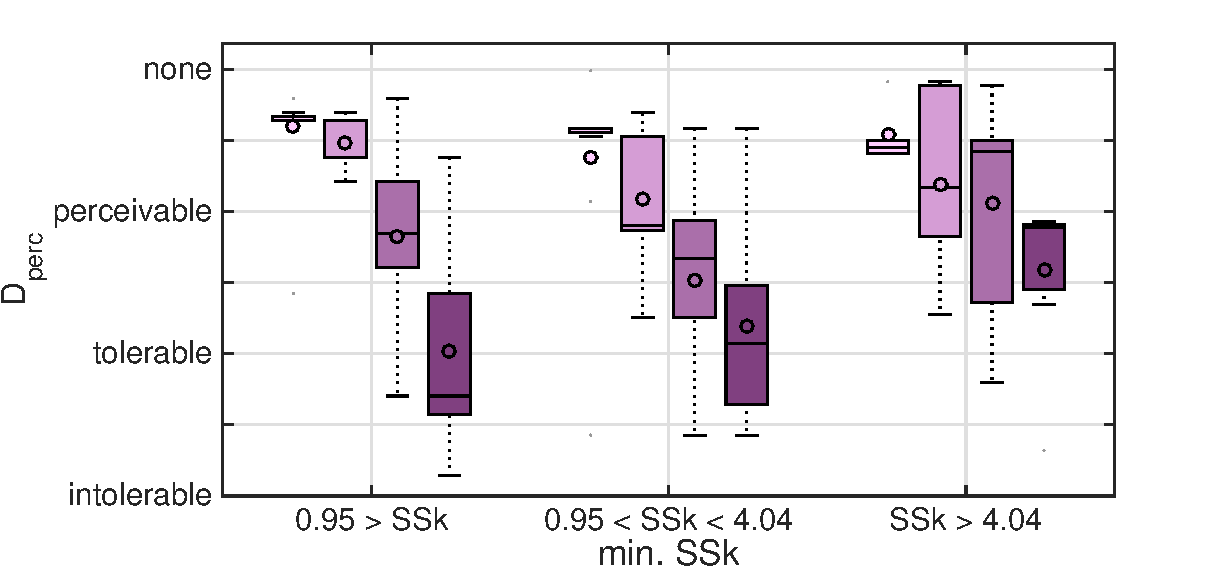
\includegraphics[width=.77\textwidth]{img/NMP/minSSk_PD}\label{fig:NMP:minSSk_SubjPerc}}  \hfil
  \subfloat[Average BPM Linear Slope $\kappa$]{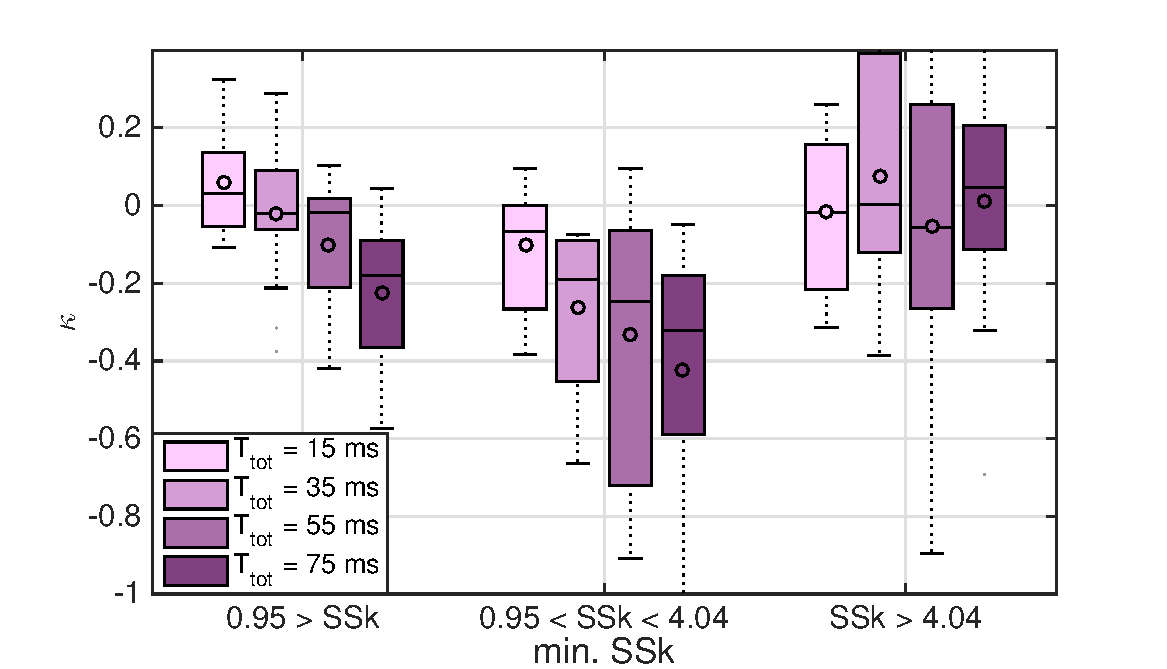
\includegraphics[width=.72\textwidth]{img/NMP/minSSk_BPM}\label{fig:NMP:minSSk_LinSlope}}        
\end{flushright}
\caption{Dependence of $\kappa$ and $D_{perc}$ on the minimum Spectral Skewness $SSk$ for different values of $T_{tot}$}
\label{fig:NMP:minSSk}
\end{figure}

Similar conclusions can be drawn on the dependence of the perceived delay $D_{perc}$ and the objective metrics $\kappa$ on the minimum $ED$, as depicted in Figure \ref{fig:NMP:minED}, due to the non-negligible correlation that exists between $RC$ and $ED$. 
These conclusions remain substantially unvaried if, instead of considering the minimum values of $RC$ and $ED$, we consider the maxima.
%\subsubsection{Dependency of Quality Metrics on Timbral Features}

\begin{figure}[!tb]
\begin{flushright}
  \subfloat[Subjective Perception of Delay $D_{perc}$]{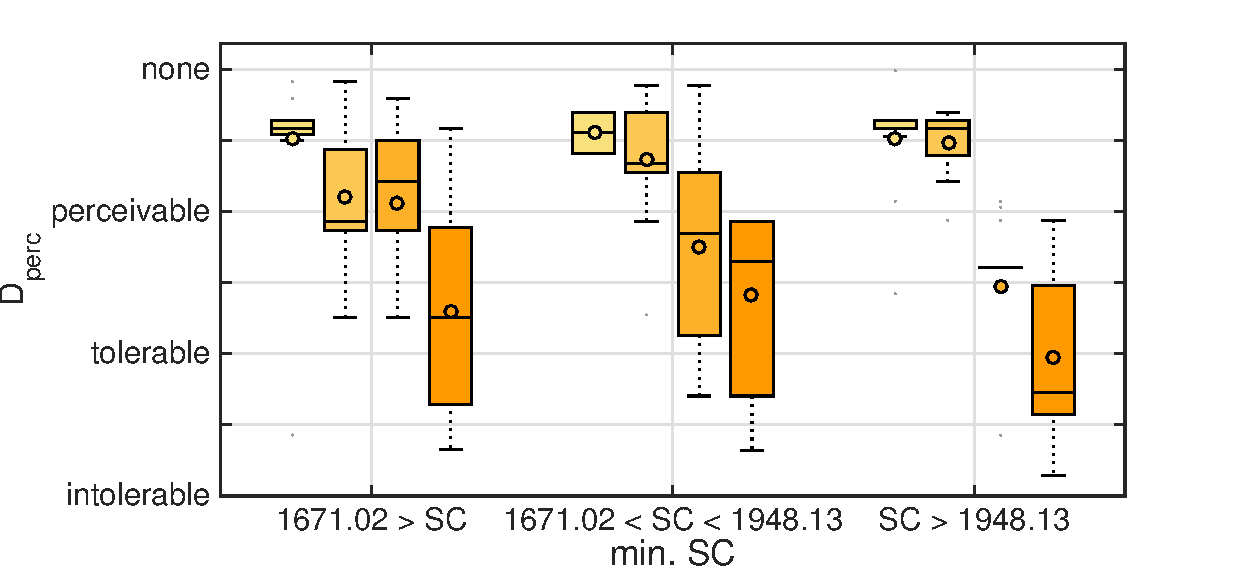
\includegraphics[width=.77\textwidth]{img/NMP/minSC_PD}\label{fig:NMP:minSC_SubjPerc}}  \hfil
  \subfloat[Average BPM Linear Slope $\kappa$]{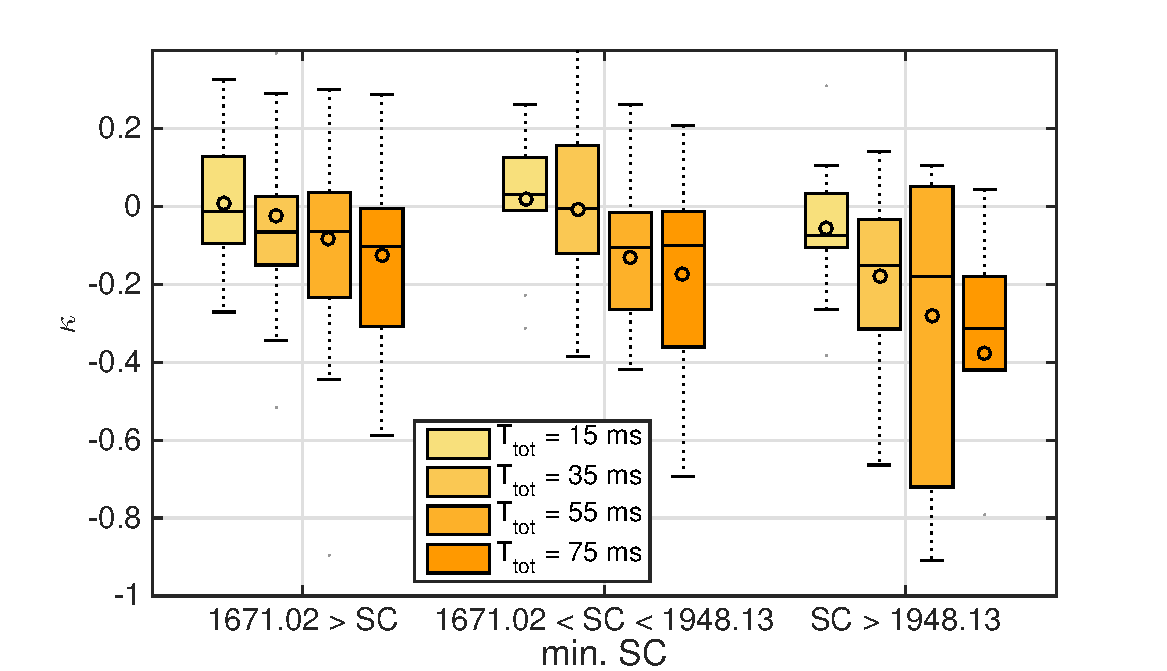
\includegraphics[width=.72\textwidth]{img/NMP/minSC_BPM}\label{fig:NMP:minSC_LinSlope}}        
\end{flushright}
\caption{Dependence of $\kappa$ and $D_{perc}$ on the minimum Spectral Centroid $SC$ for different values of $T_{tot}$.}
\label{fig:NMP:minSC}
\end{figure}


With respect to the timbral features, we observe that the noisiness of the instrument, which is captured by Spectral Entropy, Flatness and Spread, negatively affects the perceived delay $D_{perc}$. For example, in Figures \ref{fig:NMP:minSE} and \ref{fig:NMP:minSF} we show $D_{perc}$ and $\kappa$ are affected by Spectral Entropy ($SE$) and Spectral Flatness ($SF$). We consider the minimum Entropy and minimum Flatness between the two involved instruments. Focusing on the objective metric $\kappa$ (see Figures \ref{fig:NMP:minSE_LinSlope} and \ref{fig:NMP:minSF_LinSlope}), we notice that as the $SE$ and the $SF$ increase, the tempo  slowdown becomes more accentuated. This impact is negligible for low network delays, but it grows significantly for fairly large values of $T_{tot}$. Similar considerations are valid for $D_{perc}$, as reported in Figure \ref{fig:NMP:minSE_SubjPerc}. Analogous findings also apply to the dependency of the quality metrics on the Spectral Spread and here not reported for the sake of brevity.  

Conversely, when considering the impact of Spectral Skewness ($SSk$) and Spectral Kurtosis ($SK$) on the performance metrics, we notice that, for a given delay $T_{tot}$, a change in their values does not lead to a change in the quality to perceivably worsen (see Figure \ref{fig:NMP:minSSk}, results on $SK$ not reported for conciseness). 

Finally, when looking at the influence of the Spectral Centroid $SC$ (i.e., of sound brightness) on the subjective quality metrics, results reported in Figure \ref{fig:NMP:minSC_SubjPerc} show that the perceptual metric $D_{perc}$ does not exhibit significant fluctuations due to a varying $SC$. However, for large values of $SC$, a slight tendency to decelerate emerges in Figure \ref{fig:NMP:minSC_LinSlope}, which shows the impact of $SC$ on the objective quality metric $\kappa$.

It is also worth remembering that $D_{perc}$ is not necessarily an objective indicator of quality degradation of the performance, but only on the musicians' subjective perception of the end-to-end delay. For example, two musicians might keep a steady tempo ($\kappa=0$) even if they perceive a high and intolerable network delay. However, from results reported in Figures \ref{fig:NMP:minRC_SubjPerc}, \ref{fig:NMP:minED_SubjPerc}, \ref{fig:NMP:minSE_SubjPerc}, \ref{fig:NMP:minSF_SubjPerc}, \ref{fig:NMP:minSSk_SubjPerc}, \ref{fig:NMP:minSC_SubjPerc}, we can assume that such perception is strongly affected by the timbral and rhythmic characteristics of the combination of instruments and parts. For example, in Figure \ref{fig:NMP:minSSk_SubjPerc}, the perceived network delay $D_{perc}$ is higher for $SSk>4.04$ and $T_{tot}=75 ms$ than the value we would have with the same delay in the case of lower Skewness. This leads us to think that the musicians' capability of estimating the network delay is biased by the perceived interaction quality of the performance. 
This means that large network delays (i.e., $T_{tot}\geq 75ms$) do not prevent networked musical interaction, but they limit the selection of the instrument/part combinations. Thus, the resulting experience can be satisfactory if the performer is willing to trade flexibility and perceived interaction quality with the convenience of playing over the network.

\subsection{Final considerations for the Networked Music Performance}\label{sec:NMP:conclusions}
In this Section, we have discussed the ability of LLFs and MLFs representing and analyzing the music signals in the context of Networked Music Performance.
%the effectiveness of LLFs and MLFs for the formalization of the signal domain, i..e, their ability of representing and analyzing the music signals. In order to develop a better understanding of the (low-level) semantics that is carried by these features, we conducted a research activity in the context of Networked Music Performance.
This particular activity has proven that the understanding of the hand-crafted features is crucial to address the problems that regard the signal domain.  We have in fact performed an extensive evaluation of the quality of NMPs as a function of numerous parameters, some concerning telecommunication network delays and conditions, others involving rhythmic and timbral descriptors of the musical instruments involved. The analysis also considers the influence of the role of the instrument on such quality metrics.

We have found that the possibility of enjoying an interactive networked musical performance is not only a function of the total network delay, but it also depends on the role and the timbral characteristics of the involved musical instruments, as well as the rhythmic complexity of the performance. When playing more rhythmically complex pieces, musicians exhibit a more pronounced tendency to decelerate for higher network latencies. Nonetheless, the rhythmical complexity does not significantly worsen their perception of the delay and of the interaction quality.
Among the timbral features, instruments with a higher Spectral Entropy and Spectral Flatness (such as guitars and drums) lead to larger tempo slowdown in case of higher network delays. In addition, they also amplify the negative impact of network delay on the perceived delay and interaction quality.

With these results in mind, we are able to estimate the network constraints for a NMP given the combination of parts and instruments that are performing remotely.

%
%The NMP is a promising application to allow musicians to jam and compose songs from different physical location through the network. The network connections introduce a delay that musicians must take into account. While several network architectures can be proposed in order to reduce such delay, it is important to understand which factors affect the musicians' tolerance to it and which conditions make it easy for musicians to remotely perform.
%In order to conduct this analysis, we implemented a testbed for psycho-acoustic tests, which emulates the behavior of a real telecommunication network in terms of variable transmission delay and jitter. %, and we quantitatively evaluated the impact of the various performance parameters on the trend of the tempo that the musicians were able to keep during the performance, as well as on the perceived quality of the musical interaction.
%We model the analysis of factors that affect NMP as a linking function between the low-level and mid-level interpretation of the signal domain and the semantics expressed by the perceived and objective quality of the performance. The former allows us to objectively analyze the role of rhythmic complexity in the parts, as well as the timbral properties of the instruments that are played. The latter provides both a subjective and an objective evaluation of the performance. We use a manual analysis of the correlation between the two domains to understand which factors of the music performance are involved.




\section{Learned Features}\label{sec:LLFs:learned}
The hand-crafted and model-based features have been widely used in the MIR literature to extract a representation of the signal domain by employing signal processing techniques, psychoacoustic and musicological models. The use of such features requires to know in advance which characteristics are involved from the musical content and which features are able to extract such characteristics, which is not always feasible. In such situations, a typical approach is to extract all the possible features and evaluate their correlations with the desired output. However, it is possible that the features cannot extract the characteristics that matter for the specific issue and, therefore, it is necessary to identify a method to automatically extract a salient representation of the signal domain. In order to do so, we might want to mimic the human ability of organizing and elaborating the information from music.

% ----- The goal of Deep Learning -----
Recent neurological studies have shown that the human brain describes concepts (information) in hierarchical fashion \cite{Serre2007}. Indeed, the brain seems to process information through multiple stages of transformation and representation, providing multiple levels of abstraction \cite{Haykin1998}. The process is inducted by the physiological deep architecture of the mammal brain, where each level corresponds to a different area of cortex \cite{Serre2007}. As an example, in a simplistic form, while listening to a piano playing a melody, our brain first collects acoustic stimuli like frequency spectra and energy distributions. These pieces of information are then combined to build more complex concepts like the sequence of notes and the piano timbre. Notes, at the same time, are used to infer the concept of melody.

For this reason, the decomposition of decisional problems into sub-problems associated with different levels of abstraction results to be very effective \cite{Humphrey2013}. The analysis of the signal domain shall mimic this ability, but the extraction of hand-crafted features does not exploit enough depth \cite{Bengio2009}. This is why deep learning has been receiving great attention in the last few years.

Deep learning techniques attempt to emulate the human brain representation of information by providing several layers of analysis \cite{Bengio2009}. This is typically done by using a multi-layer structure such as neural networks. The input of the network represents the data under analysis (the spectrum of an audio frame in our case), and the output of each layer is a representation of the input (the \textit{learned} features in our case) obtained through processing (characteristic of the deep learning network). The more the layers, the \textit{deeper} the network and the higher the reached level of abstraction.


\begin{figure}[t]
\captionsetup[subfigure]{justification=centering}
	\centering
%      \subfloat[Input]{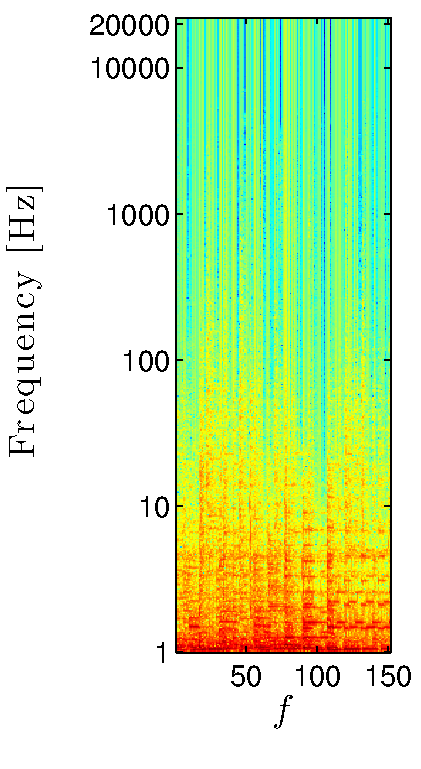
\includegraphics[width=.45\textwidth]{img/Bootleg/original_input}\label{fig:LLFs:input}} \hfil
      \subfloat[Original spectrogram]{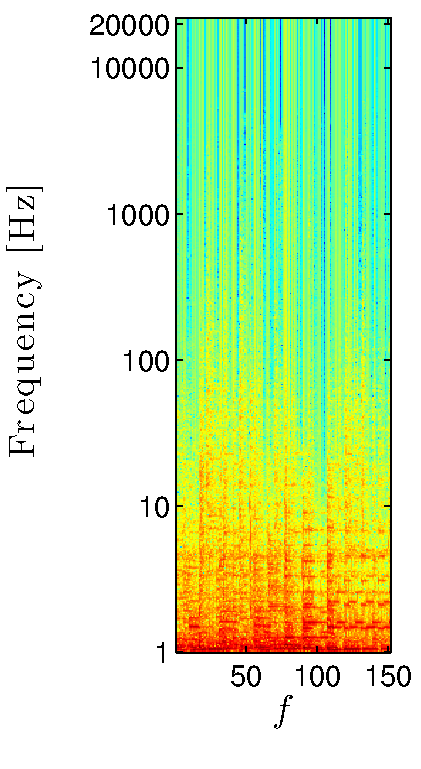
\includegraphics[trim=0cm 0cm 0cm 0cm,clip=true,totalheight=0.65\columnwidth]{img/Bootleg/original_input}\label{fig:LLFs:input}} \hfil
      \subfloat[Spectrogram reconstructed from the first layer]{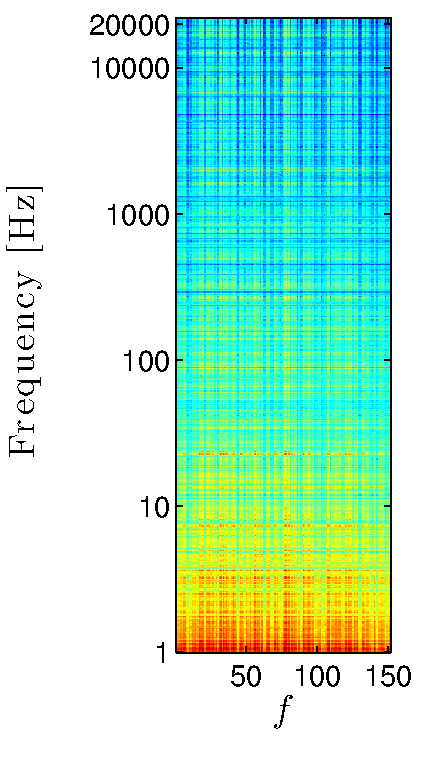
\includegraphics[trim=2.9cm 0cm 0cm 0cm,clip=true,totalheight=0.65\columnwidth]{img/Bootleg/first_layer}\label{fig:LLFs:first}}
      \subfloat[Spectrogram reconstructed from the second layer]{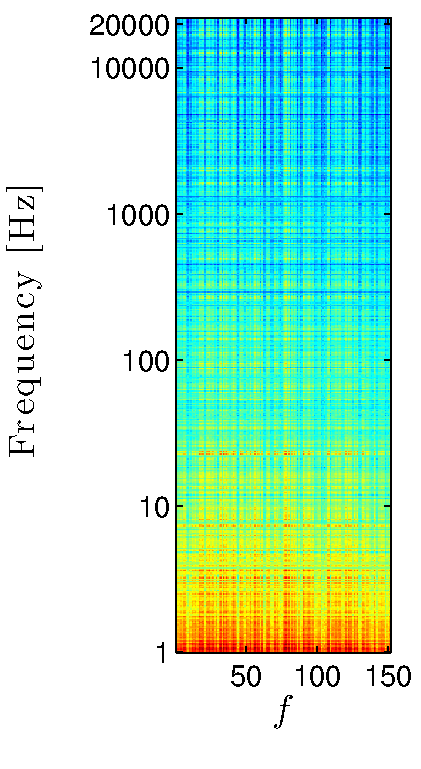
\includegraphics[trim=2.9cm 0cm 0cm 0cm,clip=true,totalheight=0.65\columnwidth]{img/Bootleg/second_layer}\label{fig:LLFs:second}}
      \subfloat[Spectrogram reconstructed from the third layer]{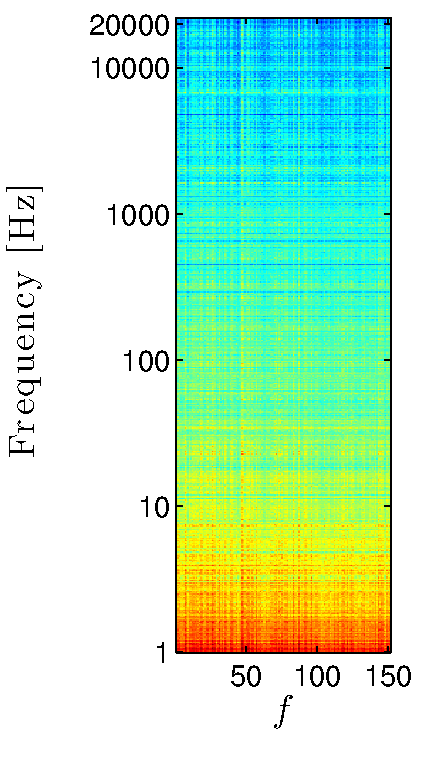
\includegraphics[trim=2.9cm 0cm 0cm 0cm,clip=true,totalheight=0.65\columnwidth]{img/Bootleg/third_layer}\label{fig:LLFs:third}}            
      \caption{A song spectrogram reconstructed from different layers of a deep learning network}
      \label{fig:LLFs:features}          
\end{figure}


Unlike hand-crafted features, features learned using deep learning methods are not easily interpretable since there is not a clear mapping with specific acoustic cues. To show the input characteristics captured by the learned features, it is possible to invert the process and reconstruct the input starting from the features. As an example, Figure \ref{fig:LLFs:features} shows a song spectrogram, and its reconstructed versions starting from learned features at different abstraction layers. We notice that, at each layer, only characteristic frequencies of the spectrum are preserved, whereas less informative bands tend to be discarded. It is also possible to further process the reconstructed spectrograms and to obtain a reconstructed waveform. In \cite{choi2015auralisation}, the authors perform an \textit{auralization} of single neurons in order to empirically infer which properties the neurons captured. Some examples of interpretation include onset detector, kick drum detector and bass note selector. 

Deep learning techniques perform non-linear transformations to input data in order to learn and extract salient information. Such techniques do not need to know in advance the target application of the extracted features, and therefore they extract a generic representation of the distribution of the input domain. For this reason, such techniques are named \textit{unsupervised} deep learning techniques, and the extracted features are referred to as \textit{unsupervised learned features}. Nevertheless, deep learning network can be also \textit{fine-tuned} in order to learn a target-oriented representation, i.e., a representation that is more useful for a given task.
 
%In particular, unsupervised deep learning techniques are able to learn and extract salient information from unlabeled data, i.e., from generic data of which they do not know any prior perform non-linear transformations to input data in order to learn and extract salient information in an unsupervised fashion. This technique is particularly suitable for feature learning process. %Although even a one-layer unsupervised learning algorithm could extract salient features, it has a limited capacity of abstraction. For this reason, a multi-layer approach can be used. Each layer is fed using the output of the lower-layer and each layer is designed to give a more abstract representation of the previous layer activations. In this way, higher-level abstractions that characterize the input could emerge.


\begin{figure}[tbp]
	\centering
	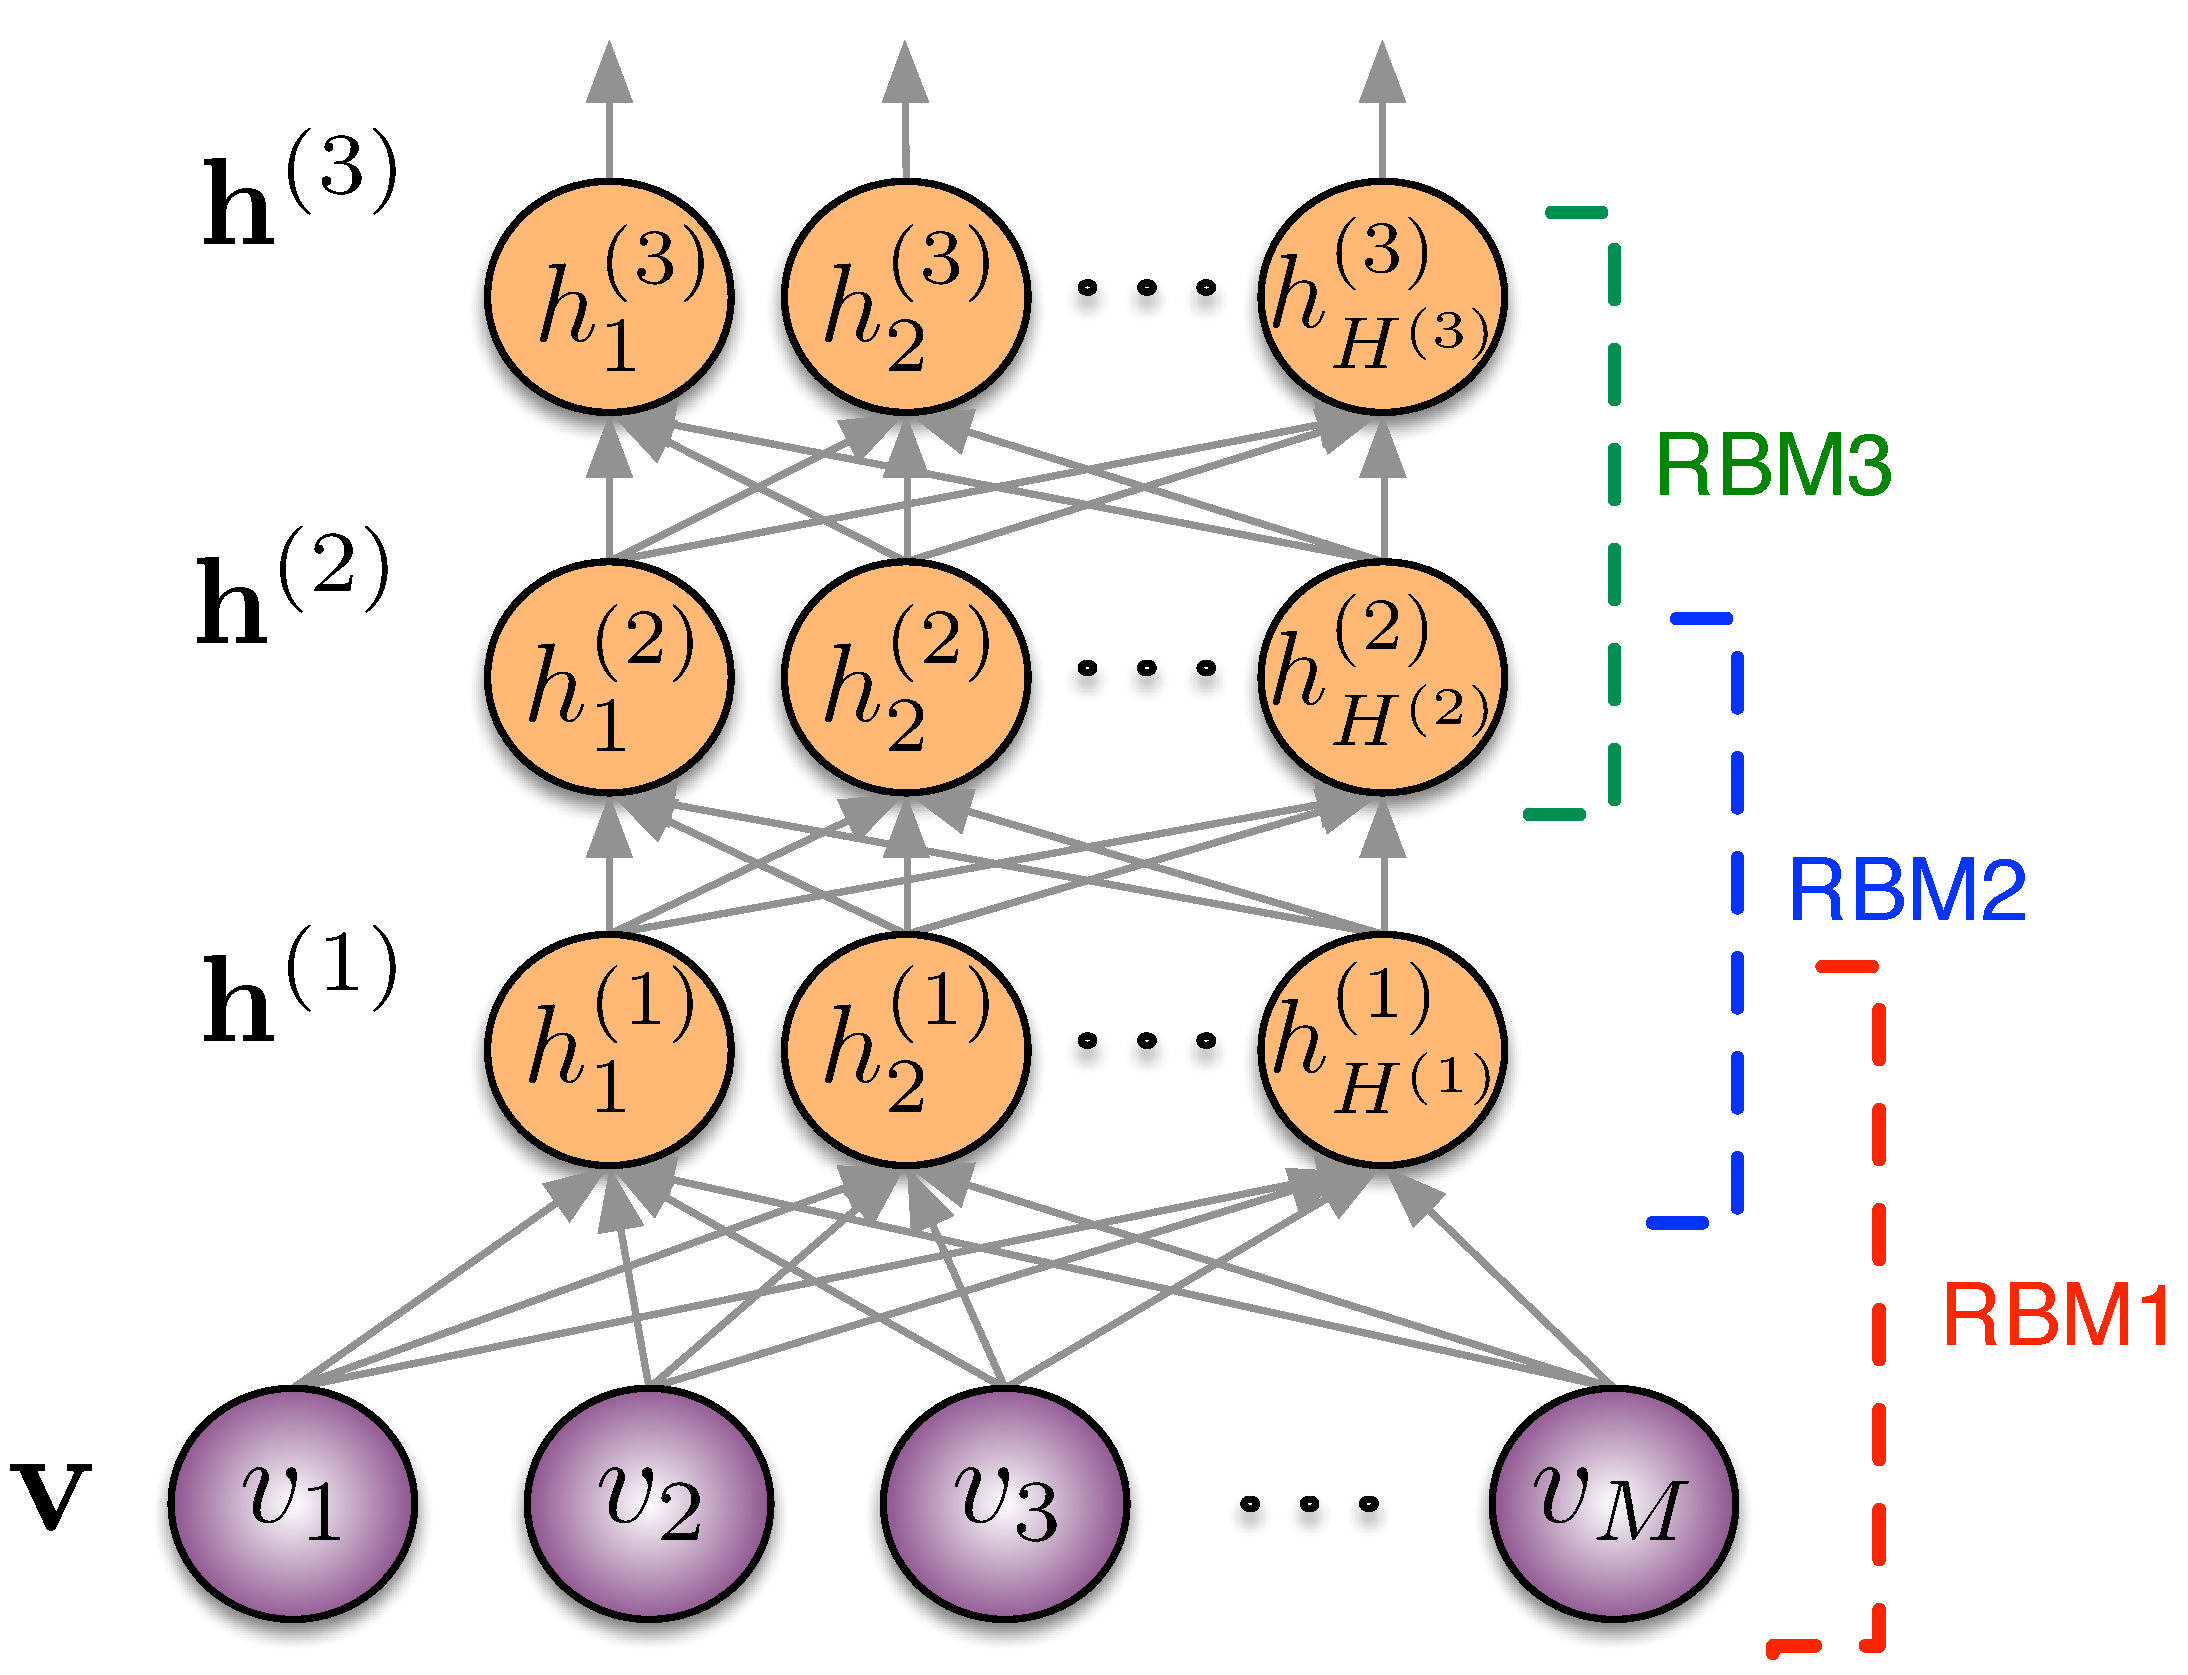
\includegraphics[width=.6\textwidth]{img/MSA/deep.pdf}
	\caption{General representation of a DBN}
	\label{fig:LLFs:DBN}
\end{figure} 


In our work we focus on a deep architecture named \textit{Deep Belief Network} (DBN), which is a multilayer neural network composed of simpler neural networks named \textit{Restricted Boltzmann Machines} (RBMs).
An RBM is a two-layer neural network that models the probability distribution of an input variable. The first layer represents the input, whose distribution is encoded by means of the second layer, which is referred to as \textit{hidden layer} \cite{Bengio2009}. The hidden layer is therefore used as a representation of the input layer.
In a DBN, a first RBM models the input distribution by means of the first hidden layer, while the second RBM models the distribution of the first hidden layer into a second hidden layer, and so on through the depth of the DBN \cite{Hinton2006}, as shown in Figure \ref{fig:LLFs:DBN} for a 3-layer DBN. Following Figure \ref{fig:LLFs:DBN}, the lowest level of the DBN, i.e., the one which learns the representation directly from the input ($\mathbf{h}^{(1)}$), is likely to learn features rather related to the signal domain, while the highest level combines the information of the lower levels of information and is able to extract more abstract information.

DBNs have been effectively employed for several tasks, such as musical genre recognition \cite{Hamel2010}, music emotion recognition \cite{Schmidt2011}, and other audio classification problems \cite{Humphrey2013}. In Chapters \ref{Chap:MSA}, \ref{Chap:Bootleg}, \ref{Chap:Violin} we present a set of application scenarios where we use the DBN architecture to automatically extract a feature representation of the signal domain with an unsupervised approach, while in Section \ref{sec:app:learned} we provide a technical overview of the RBM and DBN neural networks.

In the latest years, several other deep architectures have been proposed and tested for the representation of the signal domain. While we do not employ these architectures in our work, it is worth provide a brief overview of their use in the MIR literature.

The autoencoders, or autoassociators \cite{Bengio2009}, are a class of neural networks that use a hidden layer to learn a representation of a visible layer such that the visible layer itself can be reconstructed from the hidden layer. The hidden units are computed as a non-linear transformation of a linear combination of the input units, which can be the sigmoid function or other non-linear functions. A popular non-linear transformation is the Rectified Linear Unit (ReLU) that is defined as $f(x)=\text{max}(0,x)$, which has the advantage of being piecewise linear, hence easily tractable for the computation of the gradient \cite{Zeiler2013}. Before training an autoencoder, some noise can be added to the input, in order to avoid overfitting issues and enforce the training of the network (\textit{denoising autoencoders} \cite{vincent2008extracting}). By stacking several layers of autoencoders together, with an approach similar of the DBNs, we obtain a deep learning architecture named \textit{stacked autoencoders}. Denoising stacked autoencoders have been employed in Music Information Retrieval by \cite{maillet2009steerable} to extract a music representation for the automatic generation of playlists.

DBNs and stacked autoencoders usually work on a frame-level representation of the audio input, attempting at capturing the salient features. This approach does not take the evolution of the features over time into consideration. Two main deep architectures which include time information in the model are: the Recurrent and the Convolutional Neural Networks.

The Recurrent Neural Networks (RNNs) are able to learn a representation of the input that takes the time dimension into account by keeping memory of the past samples. In order to do so, they take as input both the data of the current frame and some information on the previous ones. More formally, given an instant $t$, which is represented by a time-frame input $x_t$, the network computes the hidden representation of the frame $h_t=f(x_t, h_{t-1})$, where $f$ is the generic function for the generation of the output (usually a non-linear function of a linear combination of the input). The presence of $h_{t-1}$ as input is important because it is itself generated as $f(x_{t-1}, h_{t-2})$, i.e., it encodes information from the previous samples \cite{mesnil2013investigation}. The RNNs are usually learned through a supervised training step to learn a representation oriented for a task. The RNNs have quickly achieved and sometimes outperformed the state-of-the-art performance in several MIR tasks, such as beat tracking \cite{bock2014multi}, music transcription \cite{sigtia2016end} or emotion recognition \cite{Weninger2014}.

The Convolutional Neural Networks (CNN) have been originally designed for image recognition and have been later used in music information \cite{lee2009convolutional}. The basic idea behind CNNs is to use a filter, named \textit{kernel}, which is convolved with the input in different locations, to collect all the outcome of such filtering and use the pooling of the outcomes as the hidden layer representation. The training step concerns the learning of the weights of the kernel, to obtain a translation-invariant hidden layer representation, due to the pooling of the filtering outcomes from different location. As an example, let us suppose that the input is a set of frames from a spectrogram: depending on the direction of the shifting of the kernel, it is possible to make a CNN either time-invariant or frequency-invariant. This addresses, for example, the problem of detecting whether a certain acoustic event occur in a spectrogram: once the kernel is learned, it will allow the CNN to capture the event in whichever moment it occurs. With the same approach, we detect frequency-shifted acoustic events. The CNNs are in fact highly flexible for the audio analysis whenever the invariance to time or frequency shifting is desirable. For this reason, CNNs have been employed for structural analysis \cite{ullrich2014boundary} as well as music classification \cite{dieleman2011audio}, annotation \cite{dieleman2014end} and recommendation \cite{van2013deep}.

Due to the tremendous impact of  deep learning on the state of the art of machine learning, many frameworks have been proposed for the design and implementation of the architectures. In this work, we use the \textit{Theano} Python library \cite{Bergstra2010}, which provides automatic gradient computation by composing and solving a computational graph derived from the architecture. Other frameworks include Caffe \cite{jia2014caffe} and TensorFlow \cite{tensorflow}.

\section{Final considerations}
The formalization of the signal domain involves the physical world of the sound waves, the perceptual world of the listening and the musicological aspects of the content. Each of this world is composed by several hierarchical layers of complexity and abstraction.

In order to extract a generic representation of the audio signal, or its musical content, we can extract LLFs or MLFs respectively. They are reliable descriptors for the signal domain, which have been manually designed by researchers to capture a specific aspect of the signal. In order to extract them, it is necessary to understand which characteristics matter for the addressing of the problem and which features can capture such characteristics. We conducted a research activity in the context of the Networked Music Performance to highlight how a deep understanding of these features can be effectively used to define the signal domain of a real problem and develop novel solutions.

However, sometimes the needed characteristics are not known in advance and the features who are supposed to capture them do not ensure the required precision. We address these issues by using the deep learning techniques to provide a generic representation of the audio signal with several layers of abstraction. Since we can hardly infer an interpretation of the learned features \cite{choi2015auralisation}, the design effort is shifted from features to architectures. Several architectures have been proposed in the literature and others can be created with ad-hoc solutions that take into account the nature of music. Nevertheless, it was proven that deep learning techniques are effective for extracting a feature representation to address problems related to the signal domain. 
